\documentclass{article}

% Includes preamble from standard file
% ==========================================================
%   GPR-20 MANUALS PREAMBLE
% ==========================================================

% ==========================================================
% Includes packages
\usepackage{float}
\usepackage{parskip}
\usepackage{caption}
\usepackage{amsmath}
\usepackage{amssymb}
\usepackage{tabularx}
\usepackage{titlesec}
\usepackage{hyperref}
\usepackage{setspace}
\usepackage{graphicx}
\usepackage{csvsimple}
\usepackage{xltabular}
\usepackage{subcaption}
\usepackage{indentfirst}
\usepackage[utf8]{inputenc}
\usepackage[margin=1in]{geometry}
\usepackage[type={CC}, modifier={by-nc}, version={4.0}]{doclicense}
\usepackage{subfiles}
% ==========================================================

% ==========================================================
% PREAMBLE SETTINGS
% Sets double spacing
\doublespacing

% Sets paragraph indentation
\setlength{\parindent}{1em}

% Sets paragraph skip
\setlength{\parskip}{2em}
% ==========================================================


% Adds bibliography
\usepackage[style=numeric]{biblatex}
\bibliography{biblio.bib}


% Defines command to insert name
\newcommand{\GPRManualName}{Basic Assembly Manual}

% ==========================================================
% DOCUMENT INFORMATION
\title{GPR-20: Basic Assembly Manual}
\author{Grupo de Desminado Humanitario}
\date{July 2021}
% ==========================================================

\begin{document}

\subfile{front}

\newpage
\section{Introduction}
This document presents the instructions to assembly the basic structure of the GPR-20 robot. The basic assembly assumes that all the parts and elements have been either manufactured or acquired. Assembly of the structure requires tools such as a saw, screwdrivers and pliers. A soldering iron or a heating gun is also required. Finally, the person that will build the robot must meet the appropriate safety requirements. Usage of safety gloves and goggles is strongly recommended. 

This document aims to allow an user to assembly the five basic groups of the GPR-20 robot. The five basic groups are intended to be transported into the survey location where the field setup can be executed. Basic groups are easier and more safe to transport in comparison to the fully assembled robot. The five basic groups that will be assembled are: ground support, Y-Axis, X-Axis, VNA holder and the electronics box. Table \ref{tab:basic_groups} introduces each of the basic groups and its purpose.

\begin{xltabular}{\textwidth}{|c|X|}

    
    \endfirsthead

    \endhead

    \multicolumn{2}{|c|}{\textit{Continues in next page}} \\ \hline
    \endfoot
    
    \caption{Basic groups of the GPR-20 robot.} \label{tab:basic_groups}
    \endlastfoot
    
    \hline \multicolumn{2}{|c|}{\textbf{Ground Support Group}} \\ \hline
    \raisebox{-\height}{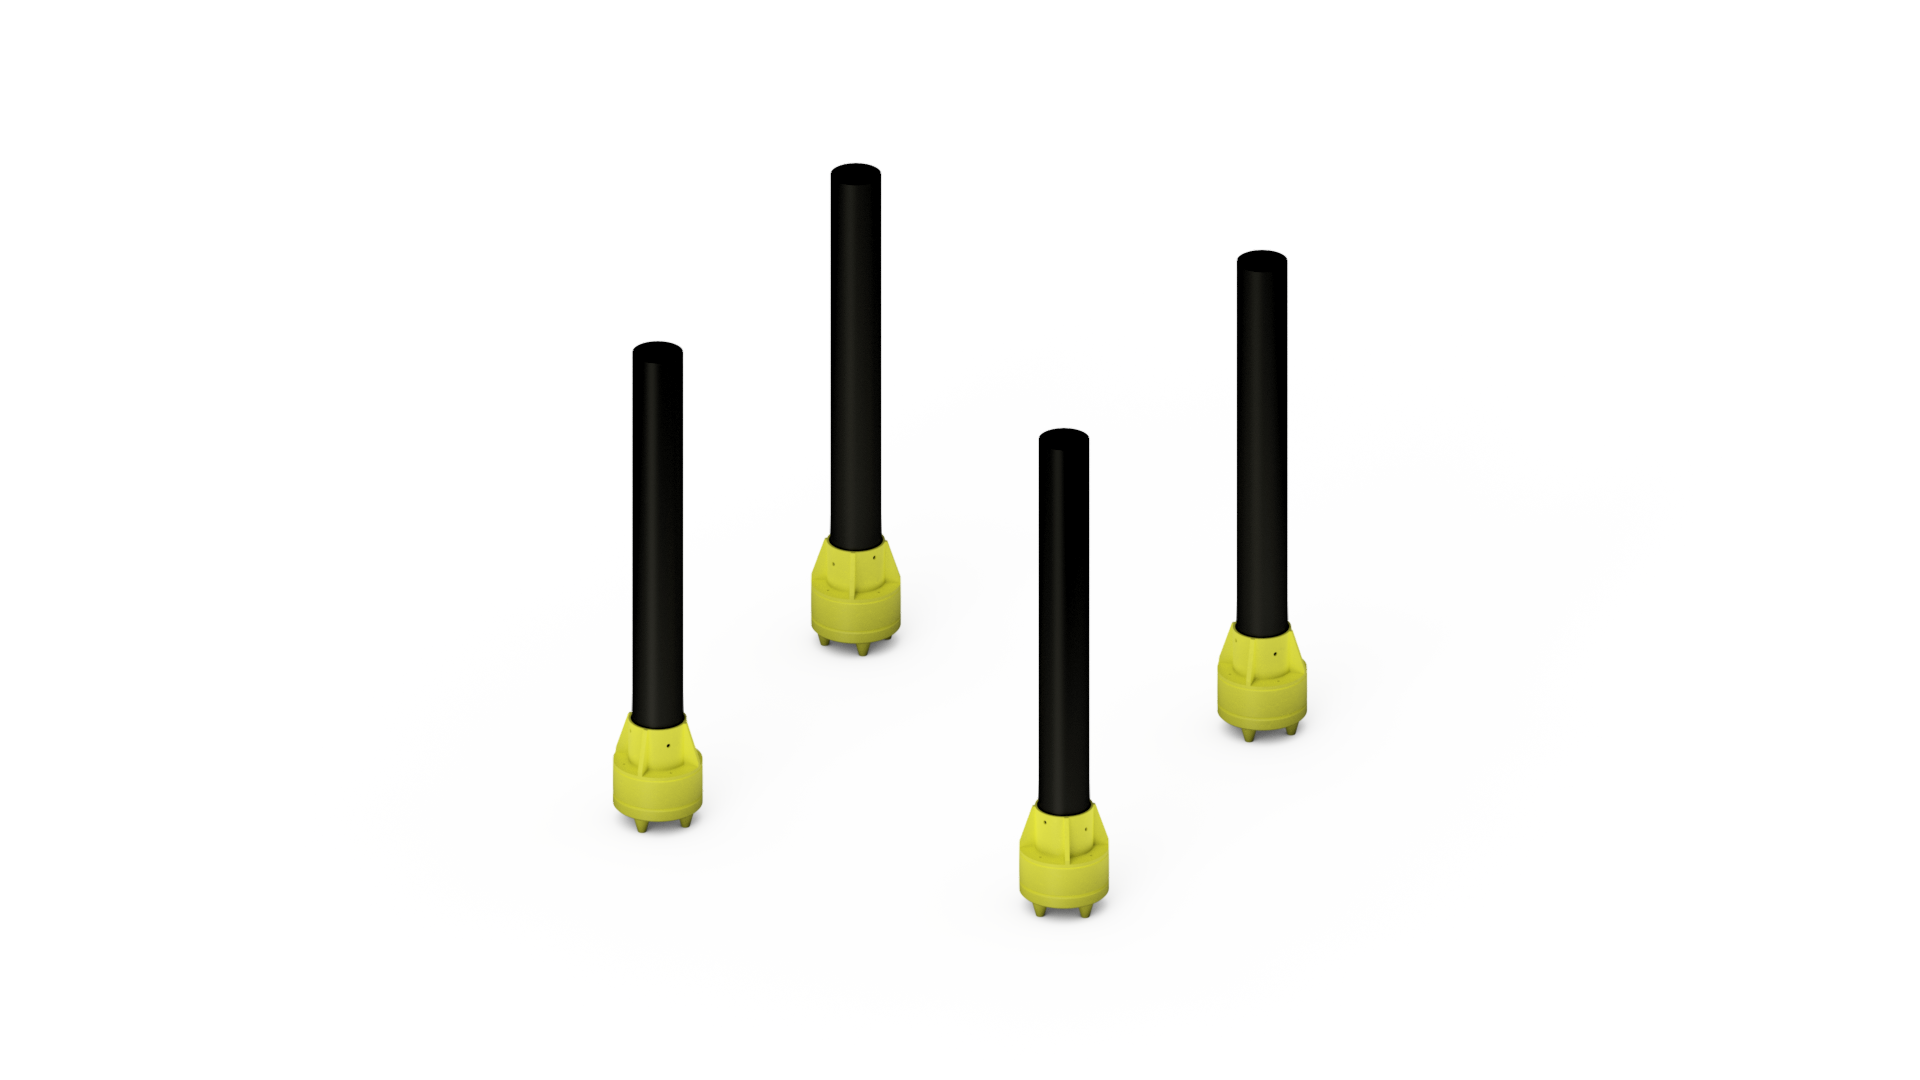
\includegraphics[width=0.4\textwidth, trim = 10cm 0 10cm 0, clip]{images/intro/ground_group.png}} & The ground support group provides the mechanical base for the GPR-20 robot. The supports can be adjusted in order to level the robot against the surface. The group consists of four equal support elements. \\ \hline
    \multicolumn{2}{|c|}{\textbf{Y-Axis Group}} \\ \hline
    \raisebox{-\height}{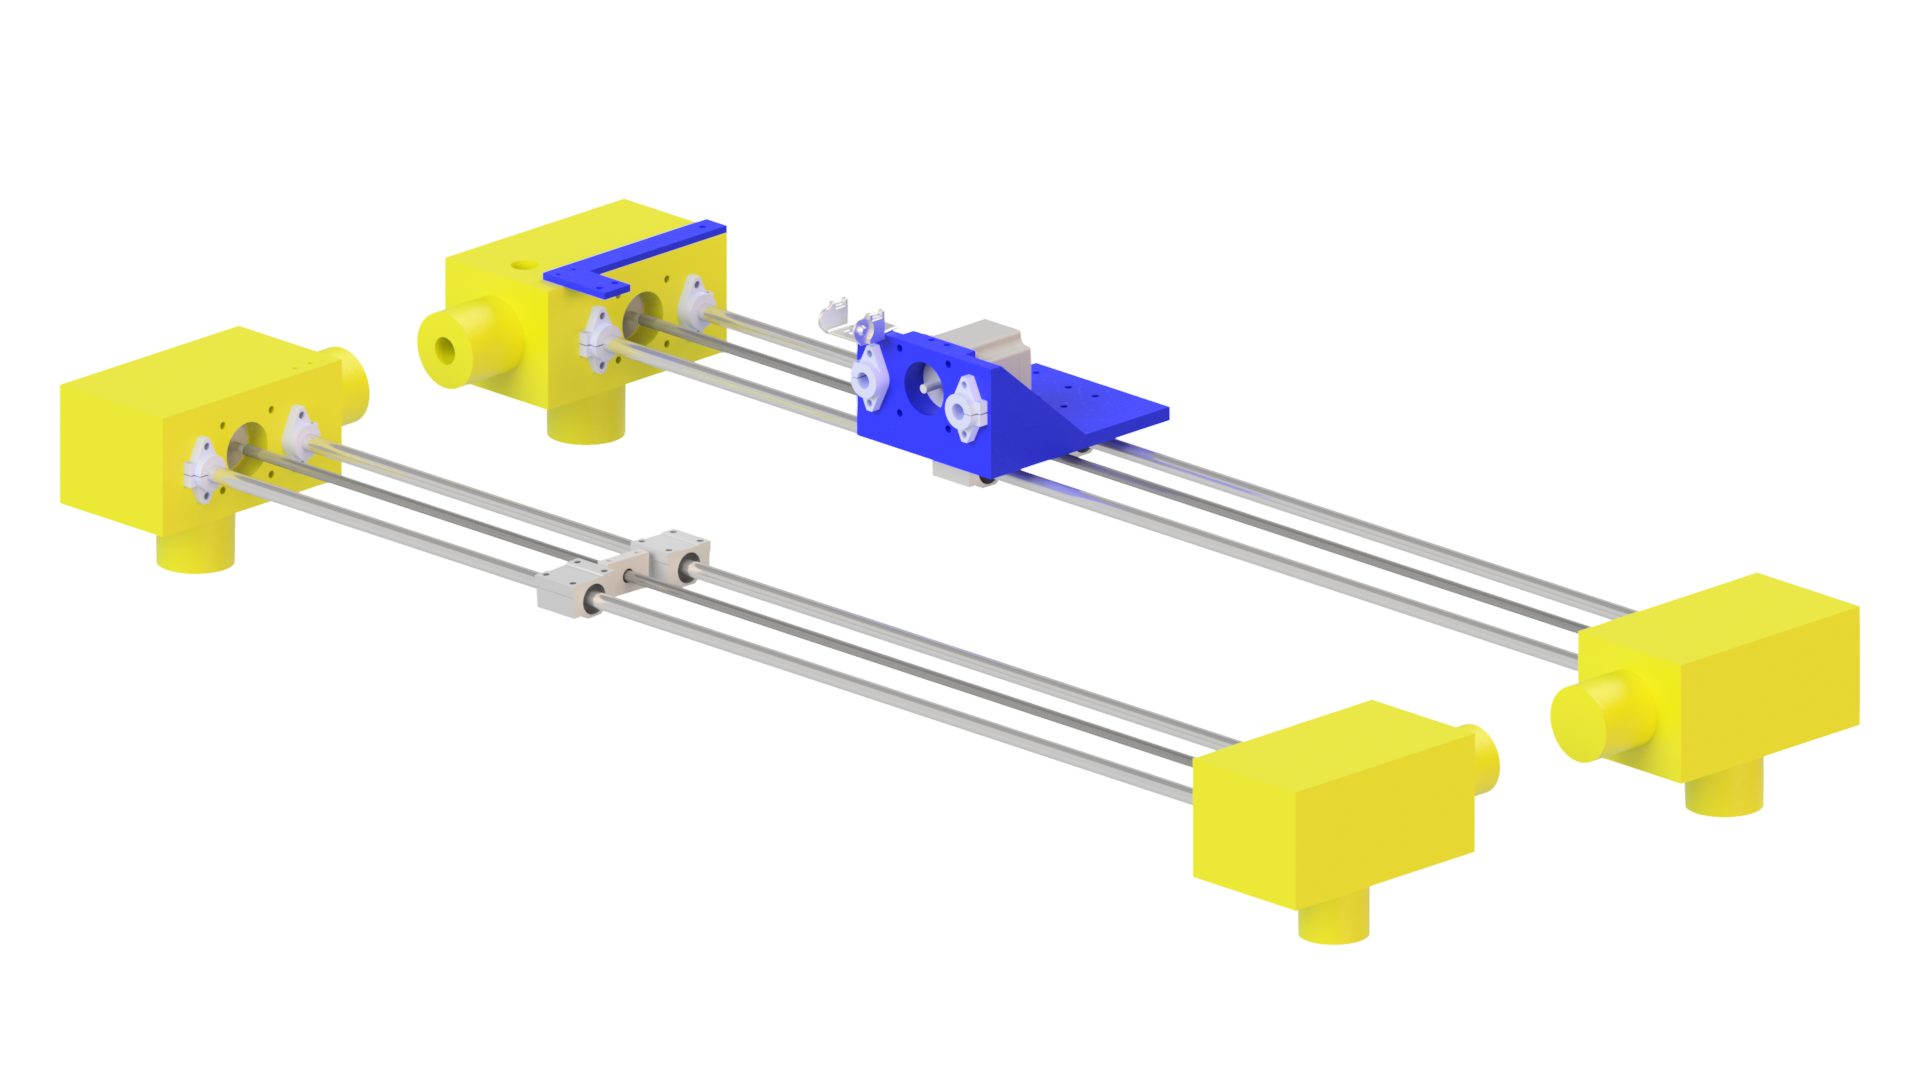
\includegraphics[width=0.4\textwidth]{images/intro/y_axes.png}} & The Y-Axis group are two linear axis that provide the movement in the Y axis direction. Both axes include a stepper motor that provides the movement for a lead screw. Both axes are equal although mirrored. The left Y axis is assembled with the driver for the X axis in order to ease the field assembly process.  \\ \hline
    \multicolumn{2}{|c|}{\textbf{X-Axis Group}} \\ \hline
    \raisebox{-\height}{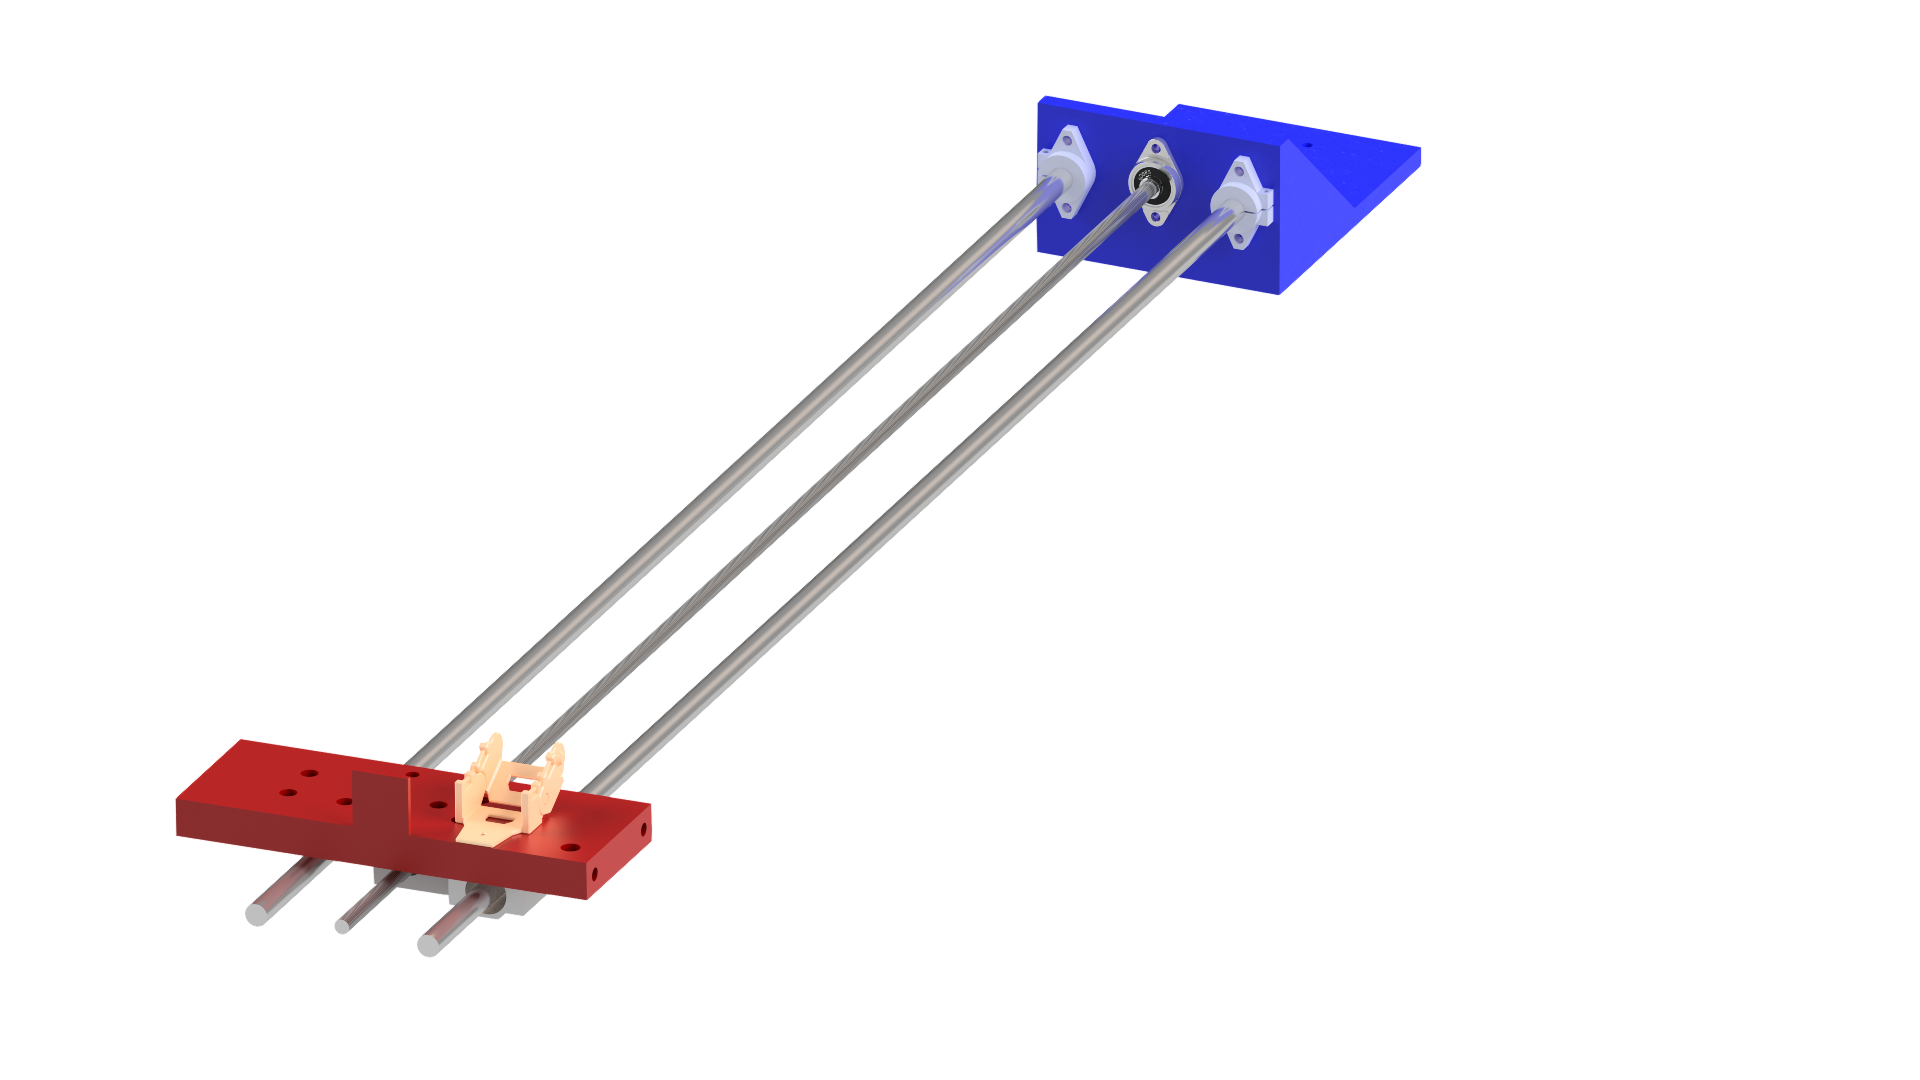
\includegraphics[width=0.4\textwidth]{images/intro/x_axis.png}} & The X-Axis group are the elements that provide the movement along the X axis direction. The X axis group includes the mount for the VNA holder group. This is done in order to ease the field assembly process. \\ \hline
    \multicolumn{2}{|c|}{\textbf{VNA Holder Group}} \\ \hline
    \raisebox{-\height}{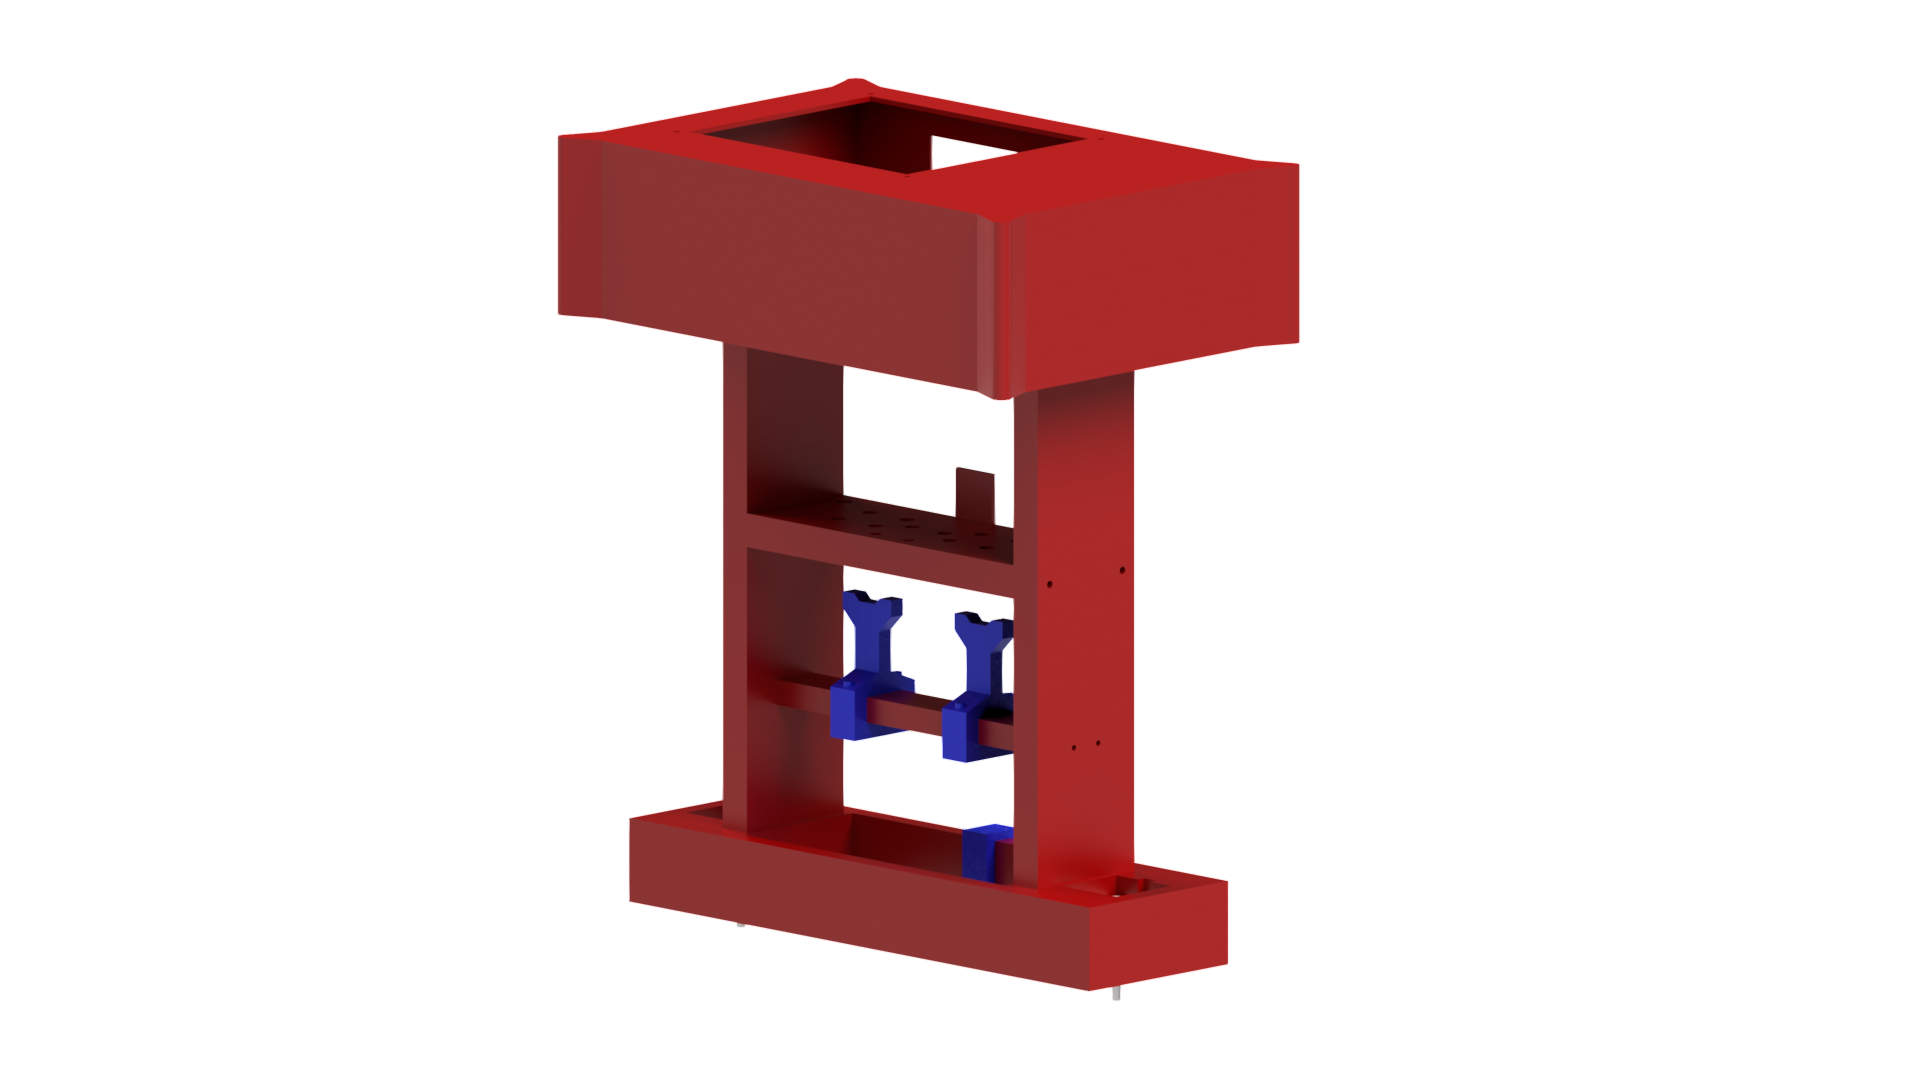
\includegraphics[width=0.4\textwidth, trim = 10cm 0 10cm 0, clip]{images/intro/vna_holder.png}} & The VNA holder group are the elements that provide the mechanical support for the Vector Network Analyzer (VNA) and the antennae. The VNA holder includes supports for two stepper motors that rotate the antennae. The height InfraRed (IR) sensor is also mounted to this group. \\ \hline
    \multicolumn{2}{|c|}{\textbf{Electronics Group}} \\ \hline
    \raisebox{-\height}{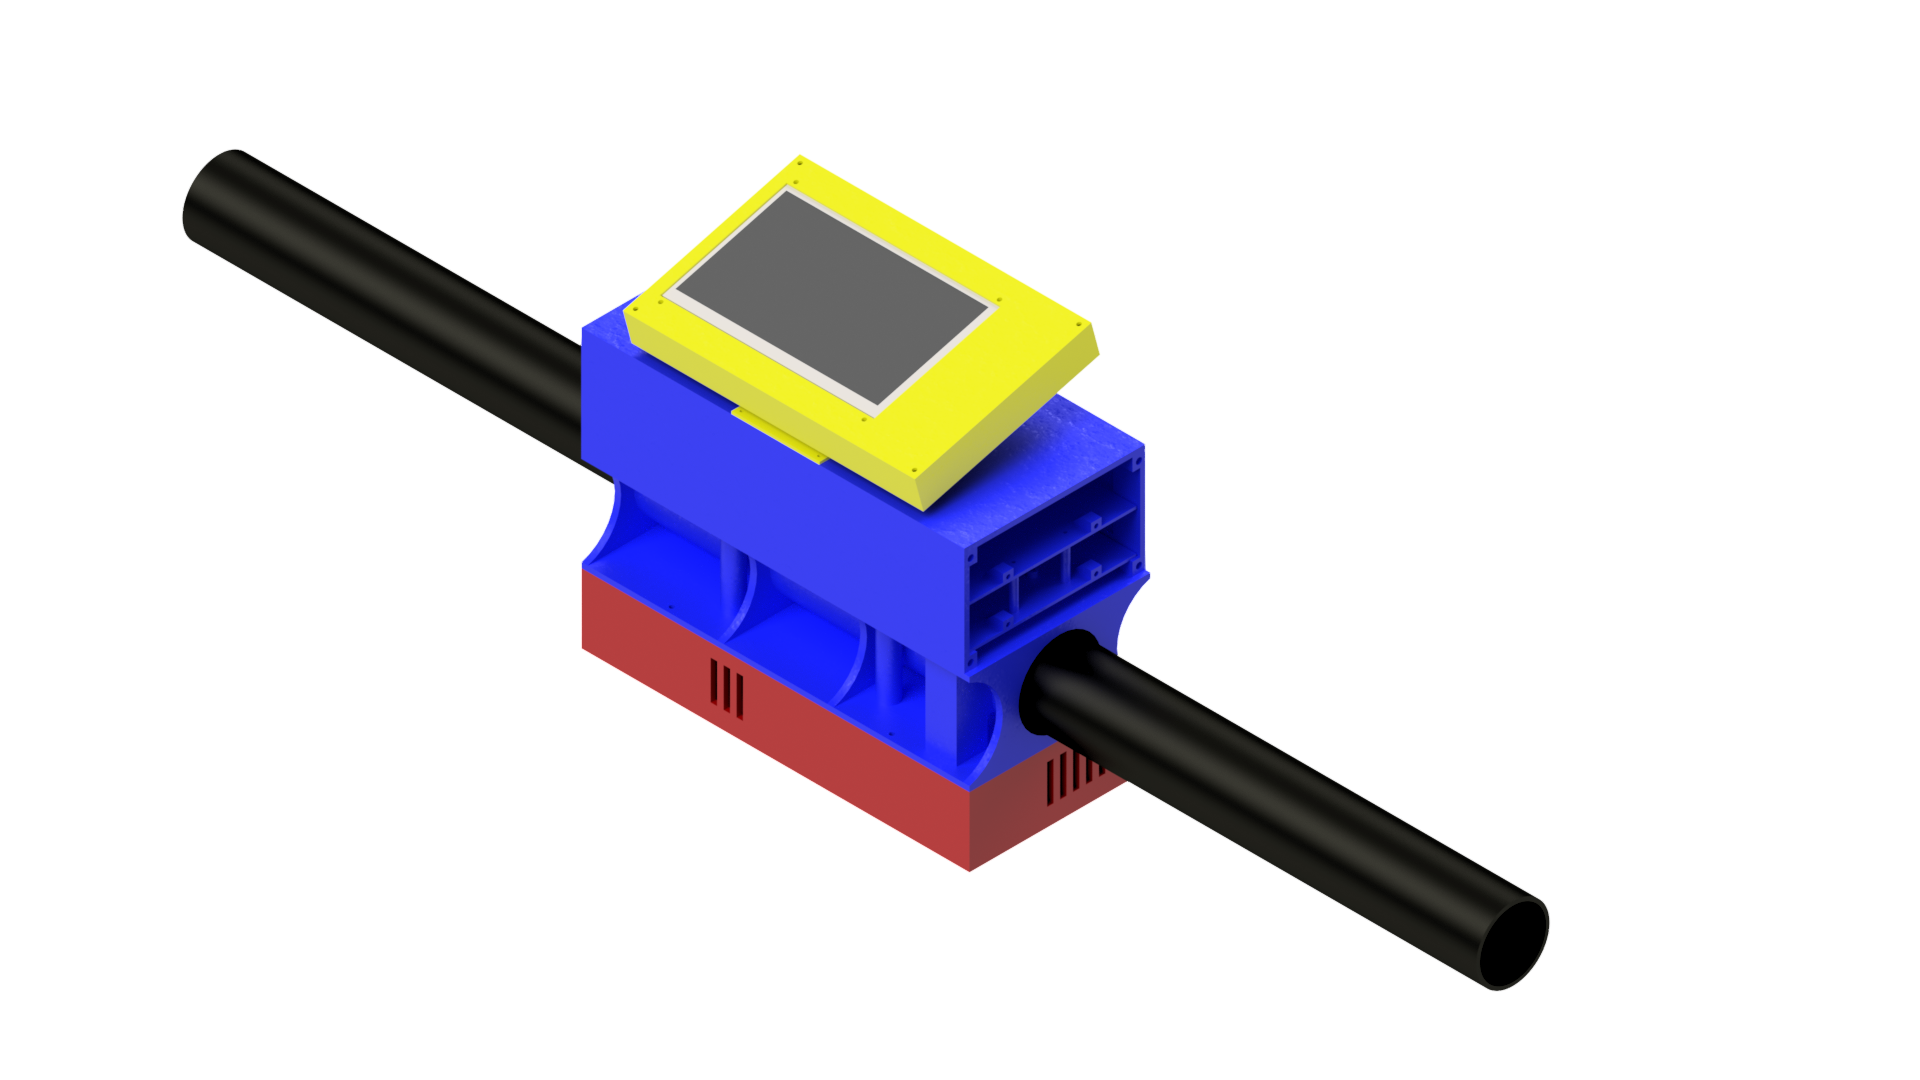
\includegraphics[width=0.4\textwidth]{images/intro/electronics_box.png}} & The electronic box are the elements that provide shelter to the electronic and power components of the GPR-20 robot. The electronics box also includes a stand for the touchscreen. \\ \hline

\end{xltabular}

\newpage
\section{Ground Support Assembly}
\begin{enumerate}
    \item Focus on the \textit{component 0} part which is shown on figure \ref{fig:gs_step_1}. You will find a hole through the part and a slot to accommodate a M7 screw nut. Put the M7 screw nut in the slot and then screw in a M7 screw from the bottom of the part. This assembly will be used later.
    
    \begin{figure}[H]
        \centering
        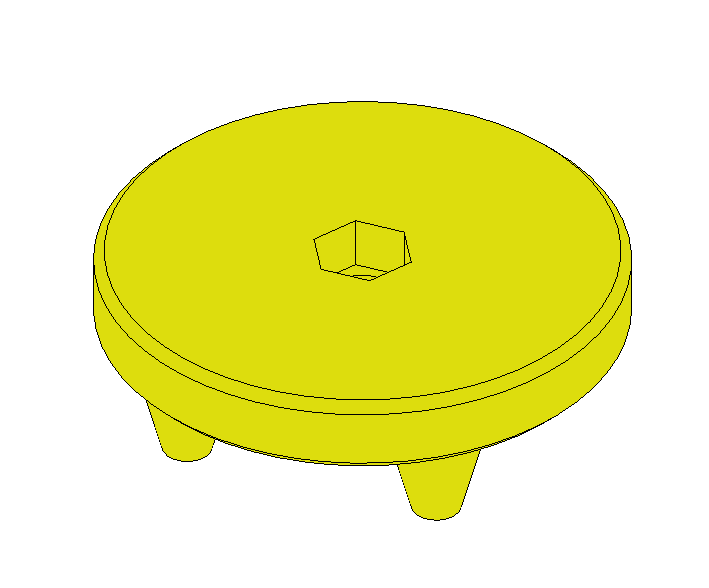
\includegraphics[width=0.5\textwidth]{images/ground/step_A.png}
        \caption{\textit{Component 0} of a ground support element.}
        \label{fig:gs_step_1}
    \end{figure}
    
    \item Focus on the \textit{component 1} part which is shown on figure \ref{fig:gs_step_2}. \textit{Component 1} has four holes that are intended to be used for M3 ($\times 4$) and M2 ($\times 4$) brass inserts. The holes for the M2 inserts are located in the inside of the part, at its bottom. The holes for the M3 inserts are located in the top of the part. Heat the brass inserts using either a heat gun or a soldering iron and place them into its corresponding holes. Allow the inserts to cool down before proceeding with the assembly.
    
    \begin{figure}[H]
        \centering
        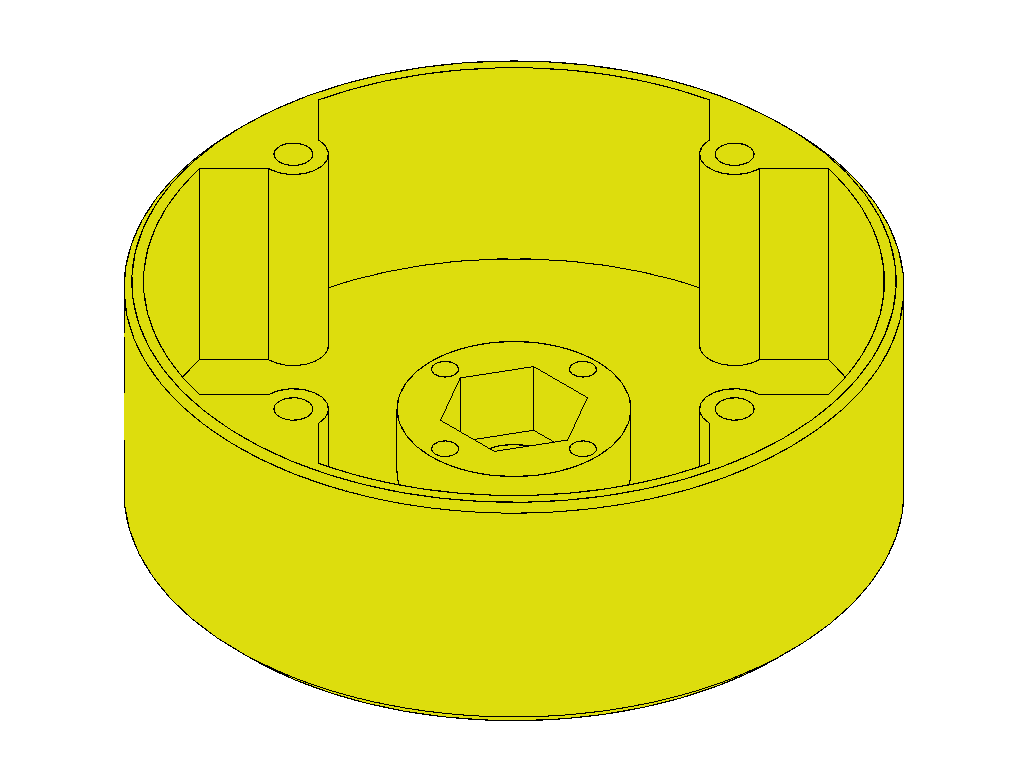
\includegraphics[width=0.5\textwidth]{images/ground/step_B.png}
        \caption{\textit{Component 1} of a ground support element.}
        \label{fig:gs_step_2}
    \end{figure}
    
    \item Place a M7 nut inside the slot of the \textit{component 1}. The M7 nut slot is located in the inside of the part, at its bottom. Use \textit{component 2} and four M2 screws to secure the nut in its place. The final assembly is shown on figure \ref{fig:gs_step_3} with \textit{component 1} in yellow and \textit{component 2} in blue.
    
    \begin{figure}[H]
        \centering
        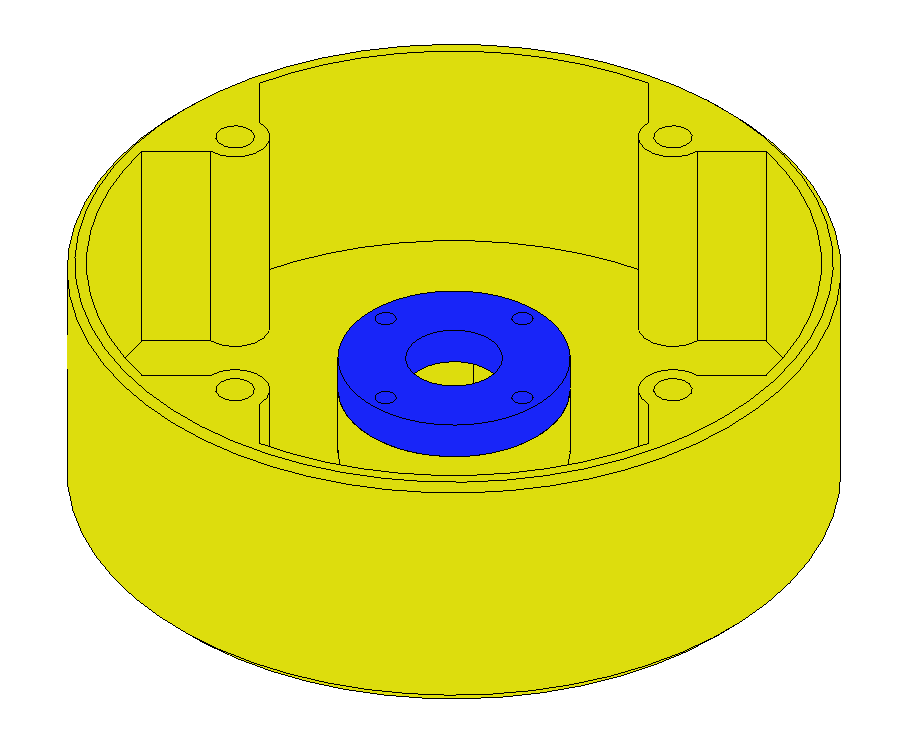
\includegraphics[width=0.5\textwidth]{images/ground/step_C.png}
        \caption{Assembly of \textit{component 1} and \textit{component 2} of a ground support element.}
        \label{fig:gs_step_3}
    \end{figure}
    
    \item Place \textit{component 3} on top of the assembly from the previous step. Use four M3 screws to secure the part. The result is shown on figure \ref{fig:gs_step_4}.
    
    \begin{figure}[H]
        \centering
        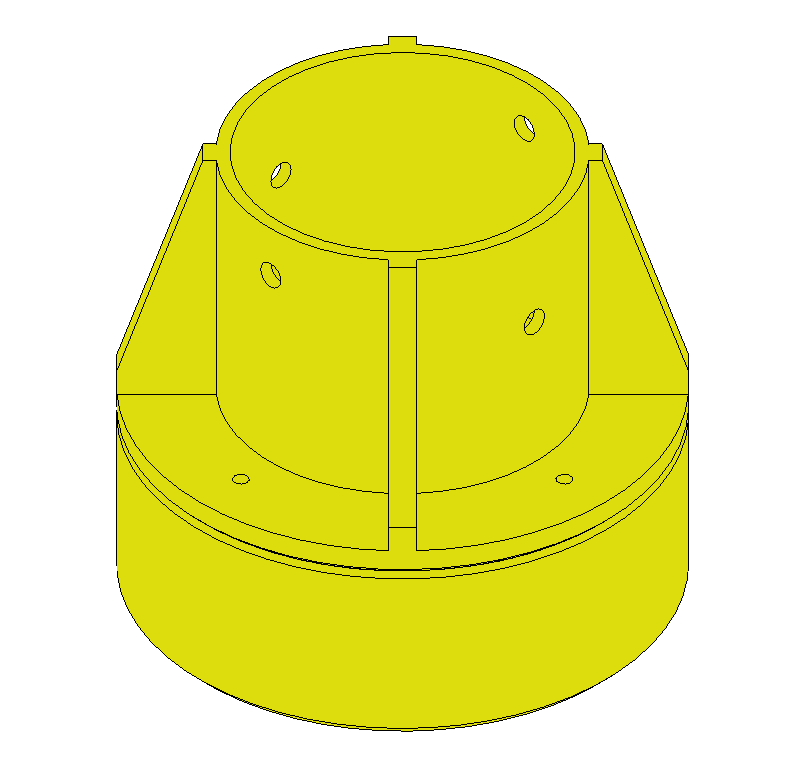
\includegraphics[width=0.45\textwidth]{images/ground/step_D.png}
        \caption{Assembly of \textit{component 1}, \textit{component 2} and \textit{component 3} of a ground support element.}
        \label{fig:gs_step_4}
    \end{figure}
    
    \item Insert the assembly from the first step into the M7 nut of the assembly from the previous step. The length of the assembly can be adjusted by rotating the M7 screw. The result of this step is shown in figure \ref{fig:gs_step_5}.
    
    \begin{figure}[H]
        \centering
        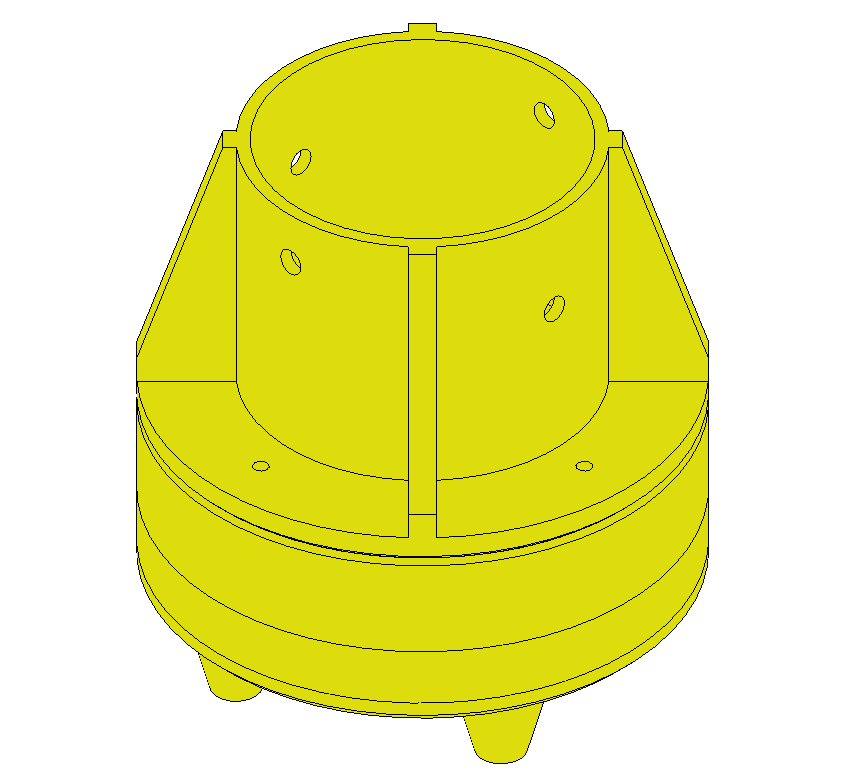
\includegraphics[width=0.5\textwidth]{images/ground/step_E.png}
        \caption{Assembly of components of a ground support element.}
        \label{fig:gs_step_5}
    \end{figure}
    
    \item Cut a two-inch ($2^{\prime \prime}$) ventilation tube to a length of fifty (50) centimeters. Insert the ventilation tube into the hole of \textit{component 3}. It is possible to use two screws to attach the tube if it is not properly secured into place by pressure. A ground support element assembly is shown on figure \ref{fig:gs_step_6}.
    
    \begin{figure}[H]
        \centering
        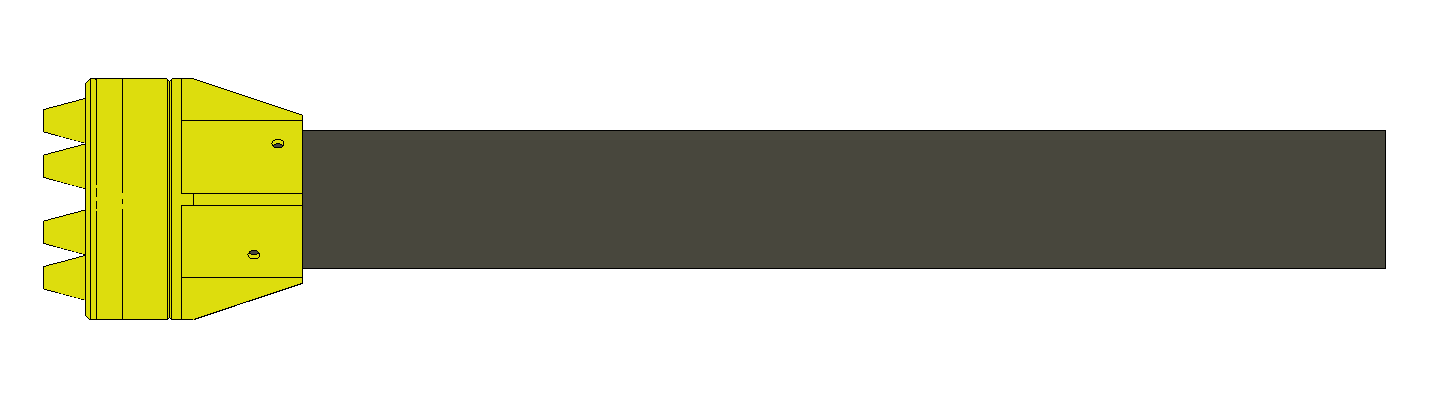
\includegraphics[width=0.9\textwidth]{images/ground/step_F.png}
        \caption{Ground support element.}
        \label{fig:gs_step_6}
    \end{figure}
    
    \item Repeat the assembly process four (4) times to fully assembly the ground support group.

\end{enumerate}

\newpage
\section{Y-Axis Assembly}
\begin{enumerate}
    
    \item Attach the NEMA23 motor to the \textit{Y-Axis left driver} element. Use four (4) M4 screws with their respective nuts. Make sure to pass the motor cables through the lateral opening of the element. The assembly is shown on figure \ref{fig:ya_step_1}.
    
    \begin{figure}[H]
        \centering
        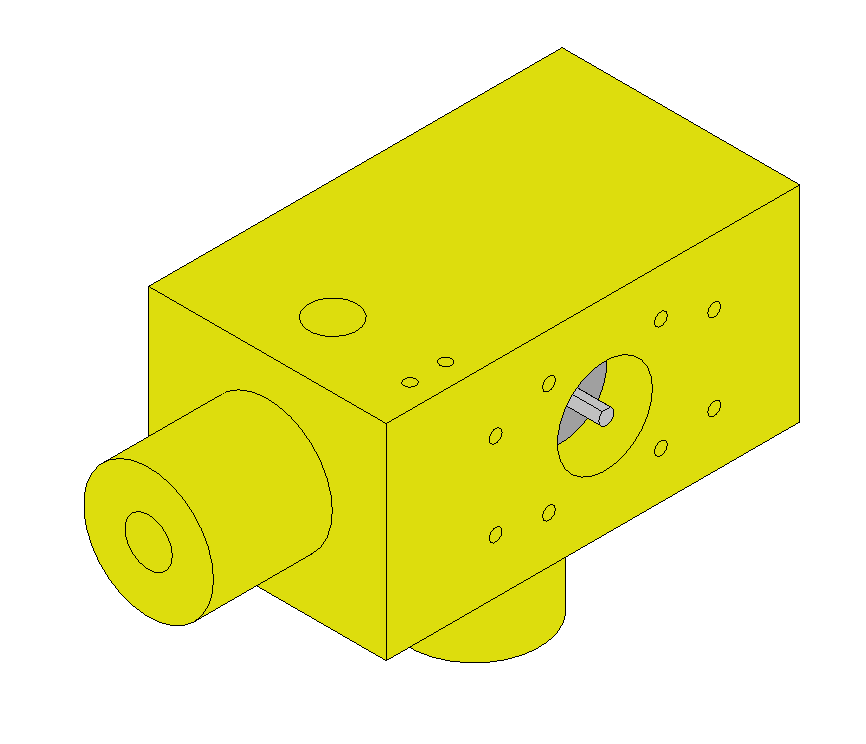
\includegraphics[width=0.45\textwidth]{images/y_axis/step_A.png}
        \caption{\textit{Y-Axis left driver} with the NEMA23 motor.}
        \label{fig:ya_step_1}
    \end{figure}
    
    \item Identify the holes in the front face of the \textit{Y-Axis left driver}. These holes are intended for four (4) M4 inserts. M4 inserts are located in the sides of the central hole. Heat the M4 inserts with a heat gun or a soldering iron and place them into their respective holes. Allow the inserts to cool down before proceeding. Attach two SHF12 linear rod support using M4 screws. Make sure to have the tightening screw facing outward. The assembly is shown on figure \ref{fig:ya_step_2}. 
    
    \begin{figure}[H]
        \centering
        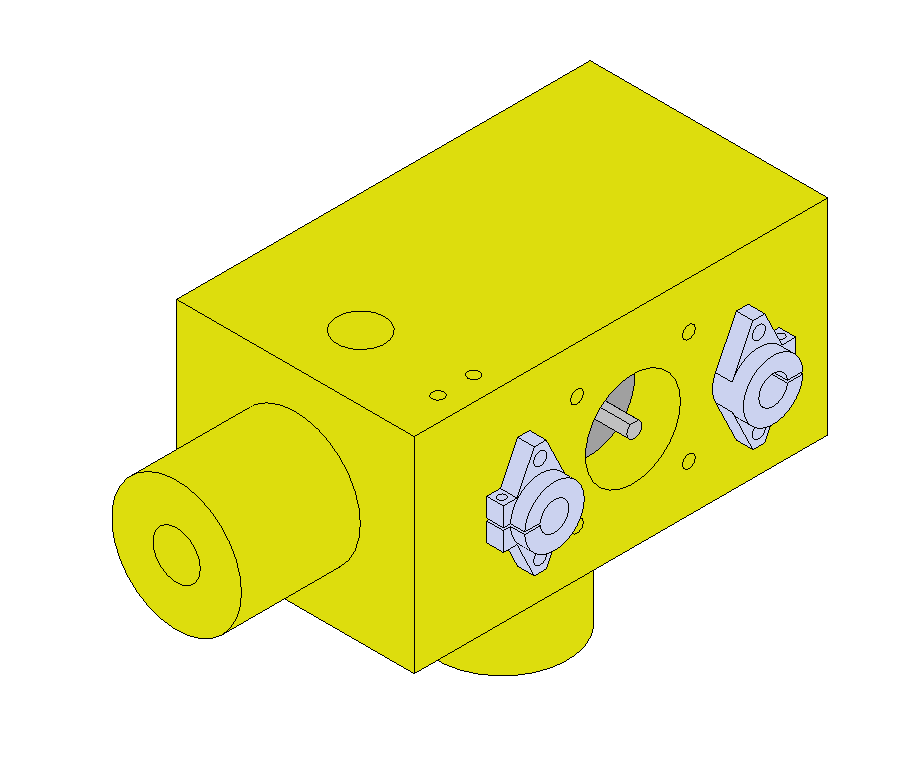
\includegraphics[width=0.45\textwidth]{images/y_axis/step_B.png}
        \caption{\textit{Y-Axis left driver} with the SHF12 supports.}
        \label{fig:ya_step_2}
    \end{figure}
    
    \item Repeat the first and second step with the \textit{Y-Axis right driver}. Mind the NEMA23 motor cables and the position of the SHF12 supports. The assembly is shown on figure \ref{fig:ya_step_3}.
    
    \begin{figure}[H]
        \centering
        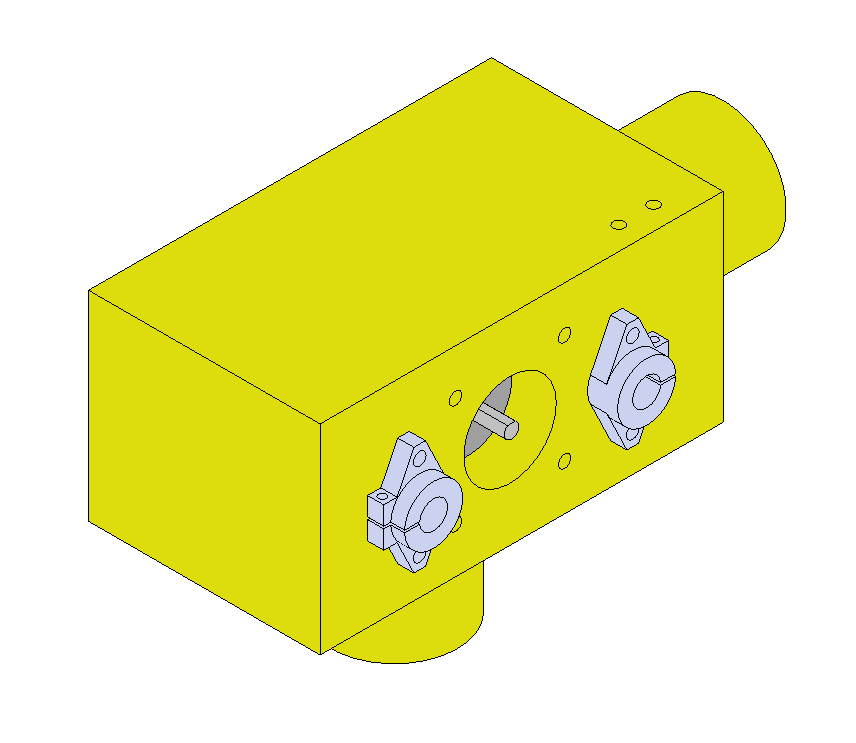
\includegraphics[width=0.4\textwidth]{images/y_axis/step_C.png}
        \caption{\textit{Y-Axis right driver} with the NEMA23 and SHF12 supports installed.}
        \label{fig:ya_step_3}
    \end{figure}
    
    \item Attach a NEMA23 motor in the \textit{X-Axis driver}. Use four (4) M4 screws with their corresponding nuts. The assembly is shown on figure \ref{fig:ya_step_4}.
    
    \begin{figure}[H]
        \centering
        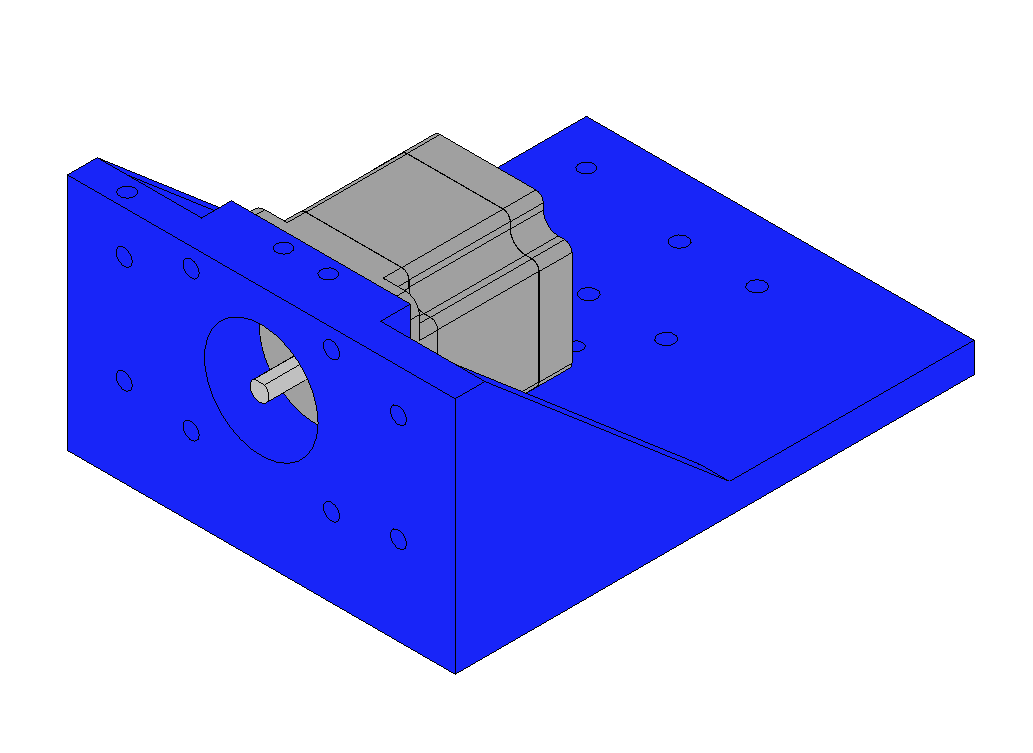
\includegraphics[width=0.4\textwidth]{images/y_axis/step_D.png}
        \caption{\textit{X-Axis driver} with the NEMA23 motor installed.}
        \label{fig:ya_step_4}
    \end{figure}
    
    \item Attach two SHF12 linear rod supports to the \textit{X-Axis driver}. Use four (4) M4 screws with their corresponding nuts. Keep the tightening screws facing outward of the component. Figure \ref{fig:ya_step_5} presents the assembly status.
    
    \begin{figure}[H]
        \centering
        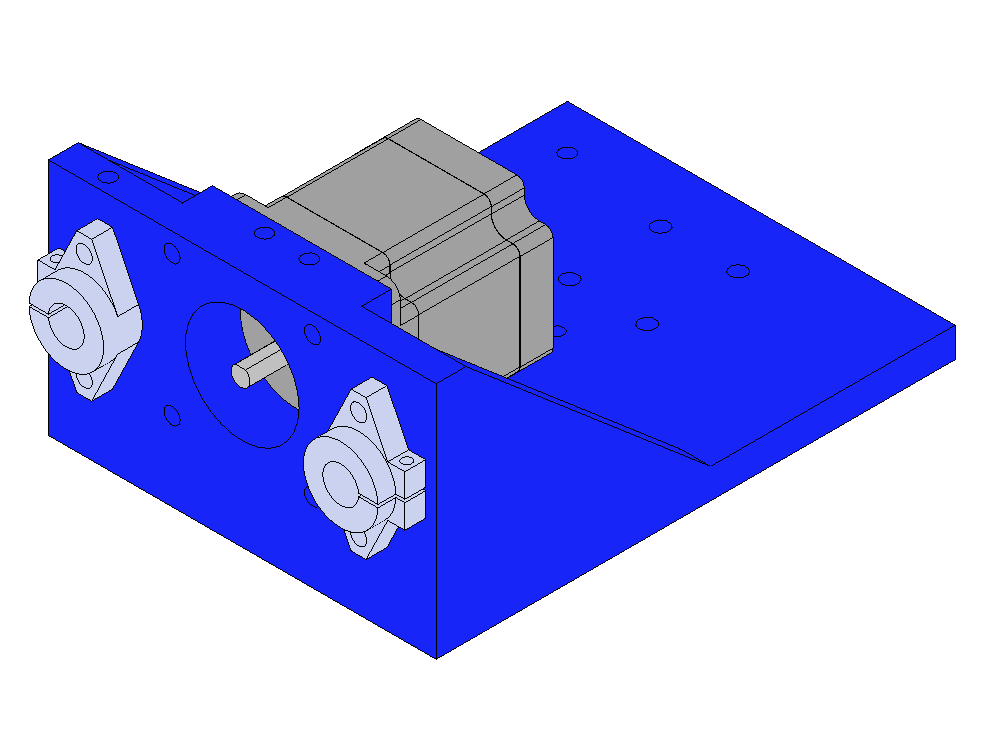
\includegraphics[width=0.4\textwidth]{images/y_axis/step_E.png}
        \caption{\textit{X-Axis driver} with the SHF12 linear rod supports attached.}
        \label{fig:ya_step_5}
    \end{figure}
    
    \item Attach two SC12UU linear rods to the bottom of the \textit{X-Axis driver} using eight (8) M5 screws. Attach the T8 nut housing to the bottom of the element using two (2) additional M4 screws with their corresponding nuts. Attach the T8 nut to the housing using four (4) M2 screws with their corresponding nuts. The assembly status is shown on figure \ref{fig:ya_step_6}.
    
    \begin{figure}[H]
        \centering
        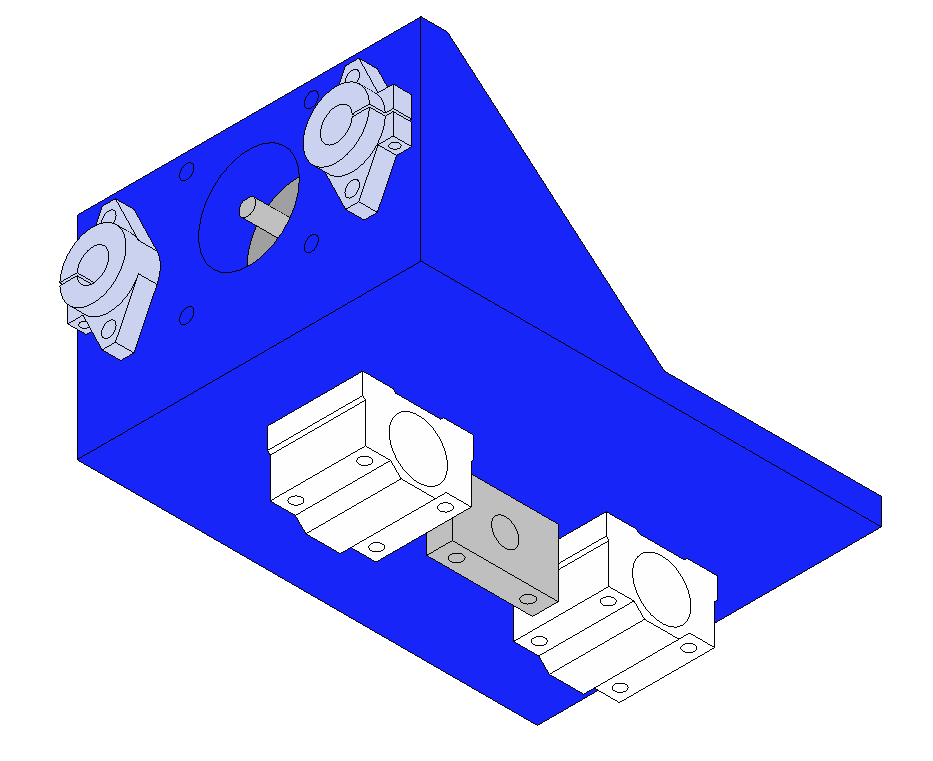
\includegraphics[width=0.4\textwidth]{images/y_axis/step_F.png}
        \caption{\textit{X-Axis driver} with the linear rod bearings and the nut housing attached.}
        \label{fig:ya_step_6}
    \end{figure}
    
    \item Consider the \textit{Y-Axis left auxiliary support} element. Notice the six holes in the fron face of the component. These holes are intended for two (2) M5 inserts and four (4) M4 inserts. The M5 inserts are located along the center of the part while the M4 screws are located at their sides. Heat the inserts with a heat gun or a soldering iron and place them into their respective holes. Make sure to place each type of insert in their correct hole. Allow the inserts to cool down before proceeding. Attach two (2) SHF12 linear rod supports and a KFL08 bearing using M4 and M5 screws respectively. Make sure to locate the SHF12 supports with the tightening screws facing outward of the element. Figure \ref{fig:ya_step_7} shows the assembly.
    
    \begin{figure}[H]
        \centering
        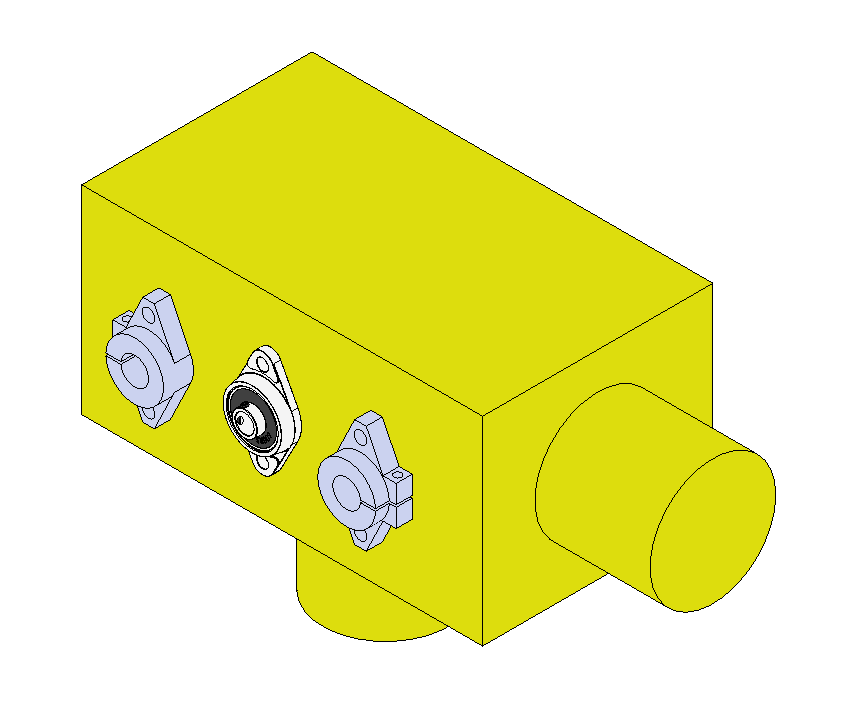
\includegraphics[width=0.4\textwidth]{images/y_axis/step_G.png}
        \caption{\textit{Y-Axis left auxiliary support} with the two (2) SHF12 supports and KFL08 bearing.}
        \label{fig:ya_step_7}
    \end{figure}
    
    \item Repeat the last step with the \textit{Y-Axis right auxiliary support}. Mind the insert type for each hole of the component and the position of the SHF12 supports. The assembly is shown on figure \ref{fig:ya_step_8}.
    
    \begin{figure}[H]
        \centering
        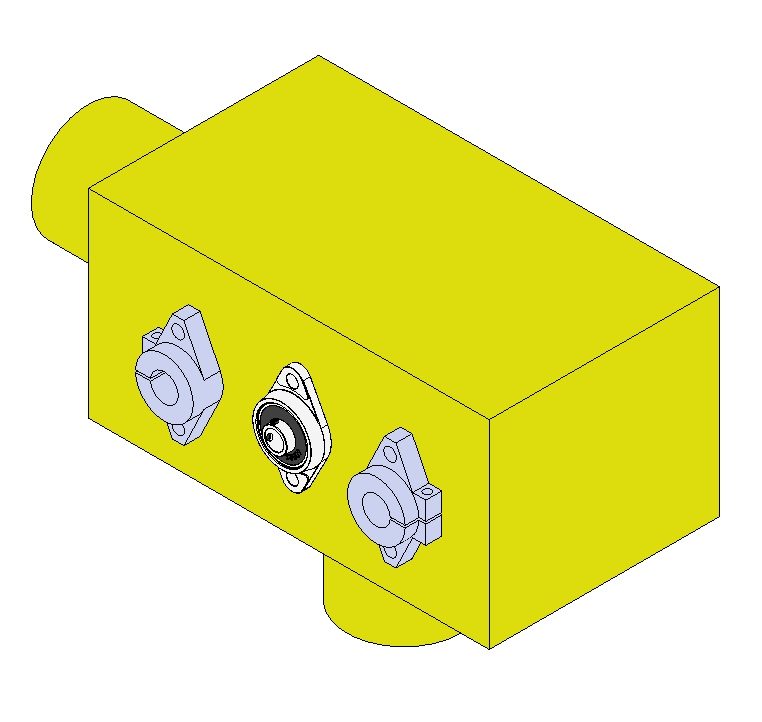
\includegraphics[width=0.3\textwidth]{images/y_axis/step_H.png}
        \caption{\textit{Y-Axis right auxiliary support} with two (2) SHF12 supports and KFL08 bearing.}
        \label{fig:ya_step_8}
    \end{figure}
    
    \item This step will make use of both the \textit{Y-Axis right driver} and \textit{Y-Axis right auxiliary support} assemblies. Attach two (2) linear rods to the SHF12 supports in the \textit{Y-Axis right auxiliary support}. Secure them by adjusting the tightening screw of the SHF12 supports. Attach the eight (8) millimeter lead screw to the KFL08 bearing and secure it by adjusting the bearing tightening screws. Roll a SC12UU bearing on each linear rod and screw a T8 nut housing with the nut installed in the lead screw. Attach the linear rods into the SHF12 supports from the \textit{Y-Axis left driver} and secure them with the tightening screws. Attach the lead screw to the motor shaft using a coupler. Figure \ref{fig:ya_step_9} presents the assembly of the right Y-Axis.
    
    \begin{figure}[H]
        \centering
        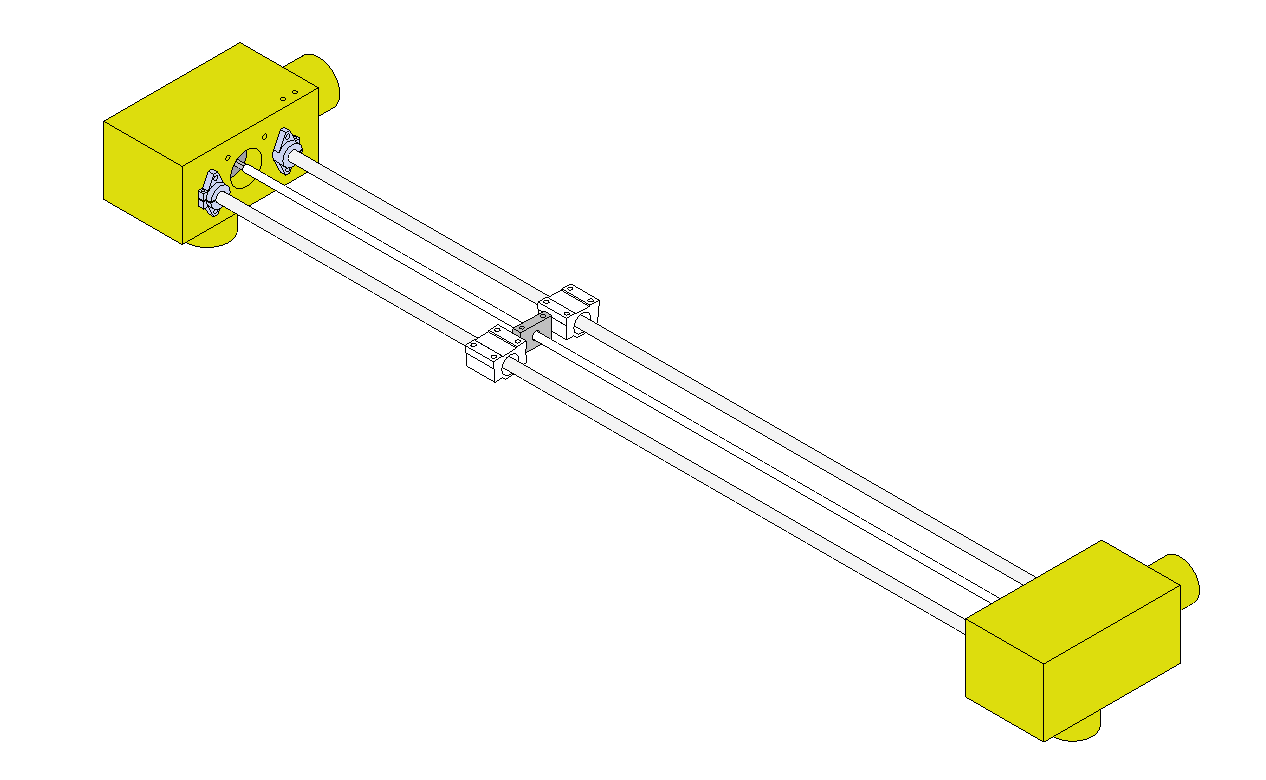
\includegraphics[width=0.6\textwidth]{images/y_axis/step_I.png}
        \caption{Right Y-Axis assembly for the GPR-20 robot.}
        \label{fig:ya_step_9}
    \end{figure}
    
    \item This step will make use of both the \textit{Y-Axis left driver}, \textit{Y-Axis left auxiliary support} and the \textit{X-Axis driver} assemblies. Attach two (2) linear rods to the SHF12 supports in the \textit{Y-Axis left auxiliary support} and secure them with the supports' tightening screws. Attach the eight (8) millimeter lead screw to the KFL08 bearing and secure it with the tightening screws. Insert the \textit{X-Axis driver} assembly into the linear rods and move it by rotating the lead screw. The \textit{X-Axis driver} must clear the linear rods in order to install the \textit{Y-Axis left driver}. Attach the linear rods to the \textit{Y-Axis left driver} and secure them with the tightening screws. Attach the lead screw to the motor shaft using a coupler. The assembly of the left Y-Axis is shown on figure \ref{fig:ya_step_10}.
    
    \begin{figure}[H]
        \centering
        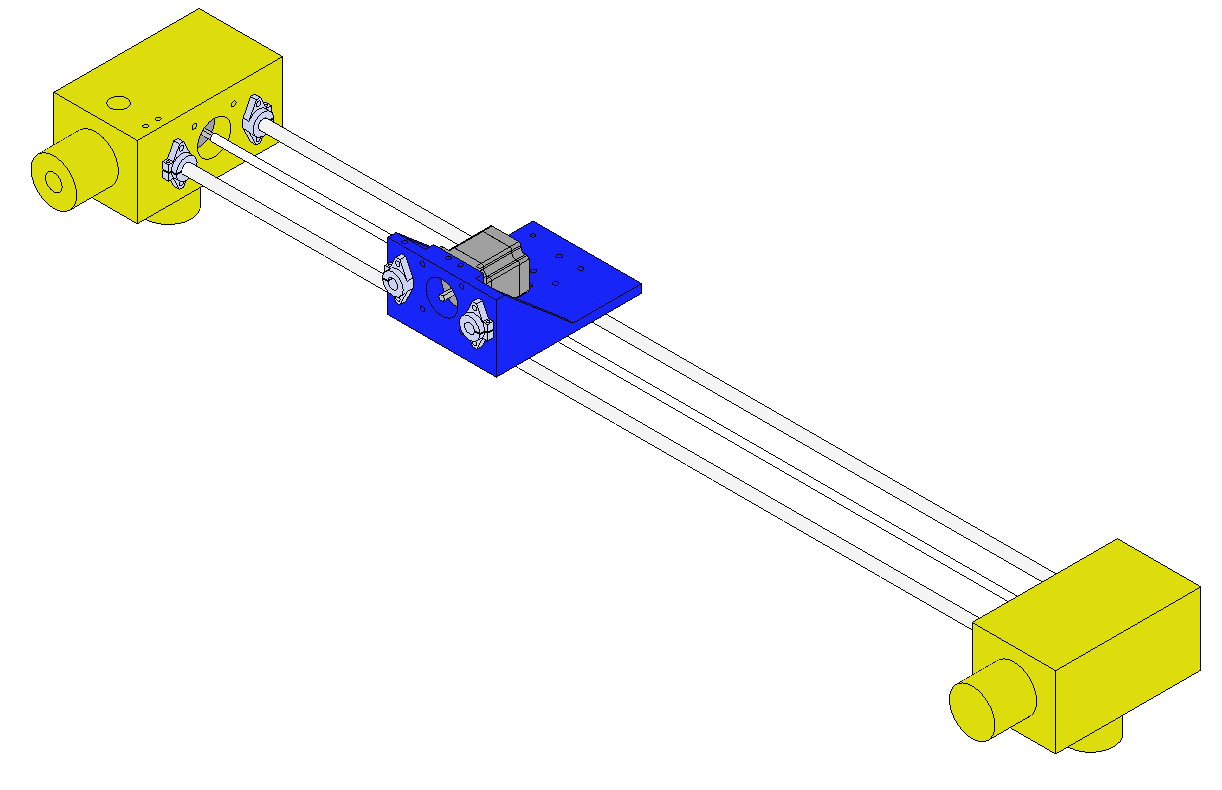
\includegraphics[width=0.6\textwidth]{images/y_axis/step_J.png}
        \caption{Left Y-Axis assembly for the GPR-20 robot.}
        \label{fig:ya_step_10}
    \end{figure}
    
    \item Identify the two (2) holes located in the top of the \textit{Y-Axis left driver}. These holes are intended for M3 inserts. Heat two (2) M3 inserts with a heat gun or a soldering iron and place them into their corresponding holes. Allow for the inserts to cool down before proceeding. Attach the \textit{Y-Axis extender} using two (2) M3 screws. The \textit{Y-Axis extender} itself has three (3) additional holes for attaching the endstop sensor and the drag chain. These holes require M3 inserts to work. Place the inserts in the three (3) holes after heating them with a heat gun or a soldering iron. The assembly is shown on figure \ref{fig:ya_step_11}.
    
    \begin{figure}[H]
        \centering
        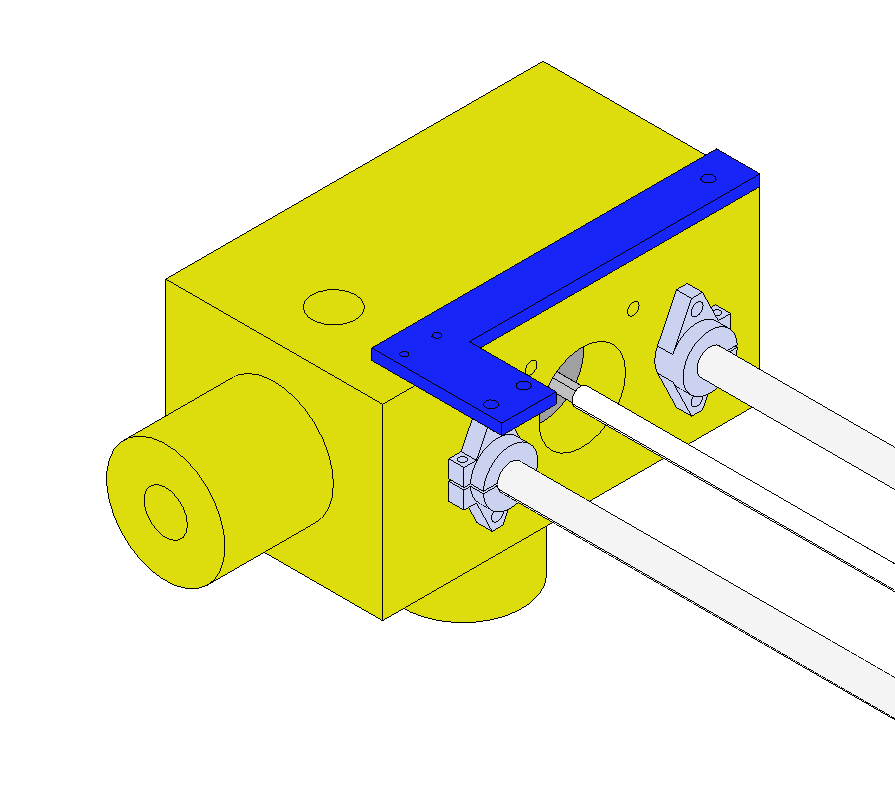
\includegraphics[width=0.4\textwidth]{images/y_axis/step_K.png}
        \caption{\textit{Y-Axis extender} attached to the left Y-Axis assembly of the GPR-20 robot.}
        \label{fig:ya_step_11}
    \end{figure}
    
    \item Identify the three (3) holes on the top of the \textit{X-Axis driver}. These holes are intended to be used by M3 inserts. Using either a heat gun or a soldering iron, heat three (3) M3 inserts and place them into the holes. Allow for the inserts to cool down before proceeding. Attach the drag chain base and \textit{X-Axis extender} to the holes using three (3) M3 screws. Place two (2) additional M3 inserts on the \textit{X-Axis extender} after heating them. Attach an endstop sensor to the extender once the inserts are cool. The assembly is shown on figure \ref{fig:ya_step_12}.
    
    \begin{figure}[H]
        \centering
        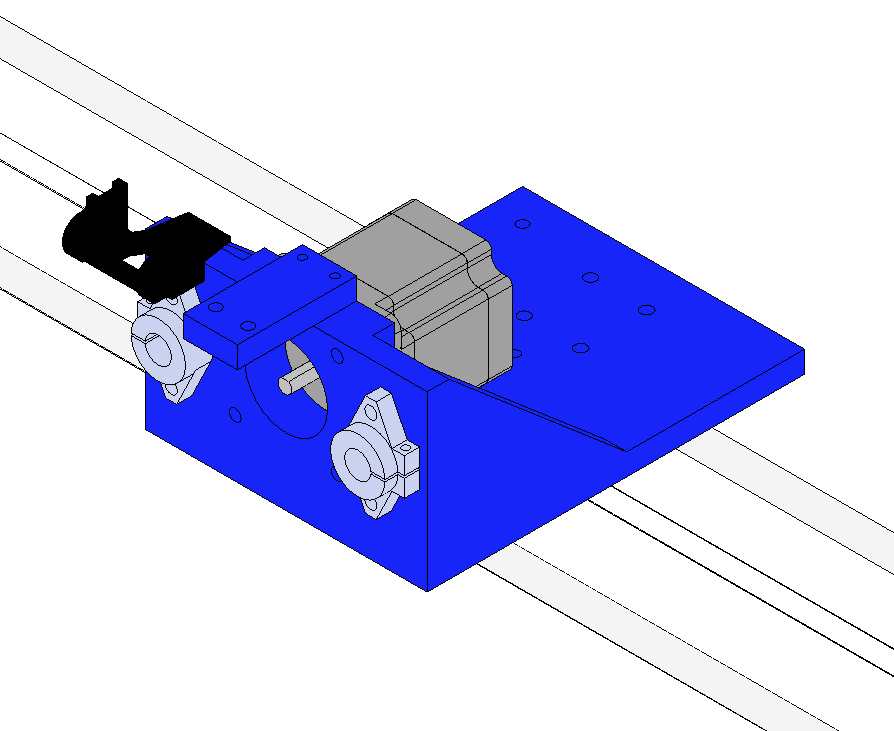
\includegraphics[width=0.4\textwidth]{images/y_axis/step_L.png}
        \caption{\textit{X-Axis extender} attached to the \textit{X-Axis driver}.}
        \label{fig:ya_step_12}
    \end{figure}
    
\end{enumerate}

\newpage
\section{X-Axis Assembly}
\begin{enumerate}

    \item Focus on the X axis auxiliary support. Attach two (2) SHF12 linear rod supports using four (4) M4 screws with their corresponding nuts. Attach the linear rod supports on the lateral holes of the driver front face. Attach a single (1) KFL08 bearing using two (2) M5 screws with their corresponding nuts. The result of the assembly is shown on figure \ref{fig:xa_step_1}. Leave the assembly for later use.
    
    \begin{figure}[H]
        \centering
        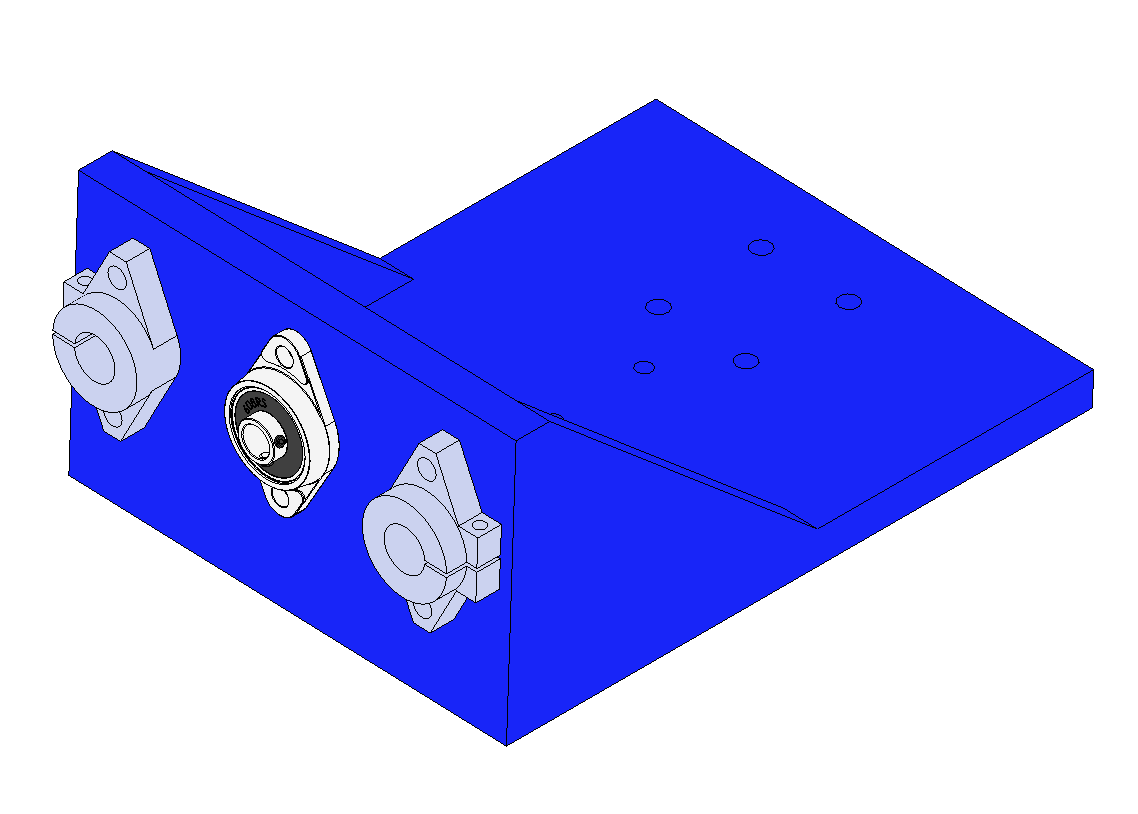
\includegraphics[width=0.5\textwidth]{images/x_axis/step_A.png}
        \caption{Assembly of the \textit{X-Axis auxiliary support} with two (2) SHF12 supports and one (1) KFL08 bearing.}
        \label{fig:xa_step_1}
    \end{figure}
    
    \item Take the \textit{universal mount} part. Identify the two (2) lateral holes in each side of the component. These holes are intended to be used by four (4) M5 inserts. Heat the inserts using a heat gun or a soldering iron and place them into the holes. Allow the inserts to cool down. Attach two (2) SC12UU bearings in the lower face of the \textit{universal mount}. Use eight (8) M5 screws. Attach a T8 nut housing using two M4 screws with their corresponding nuts. Attach the T8 nut to the housing using four (4) M2 screws with their corresponding nuts. The result of the assembly is shown on figure \ref{fig:xa_step_2}.
    
    \begin{figure}[H]
        \centering
        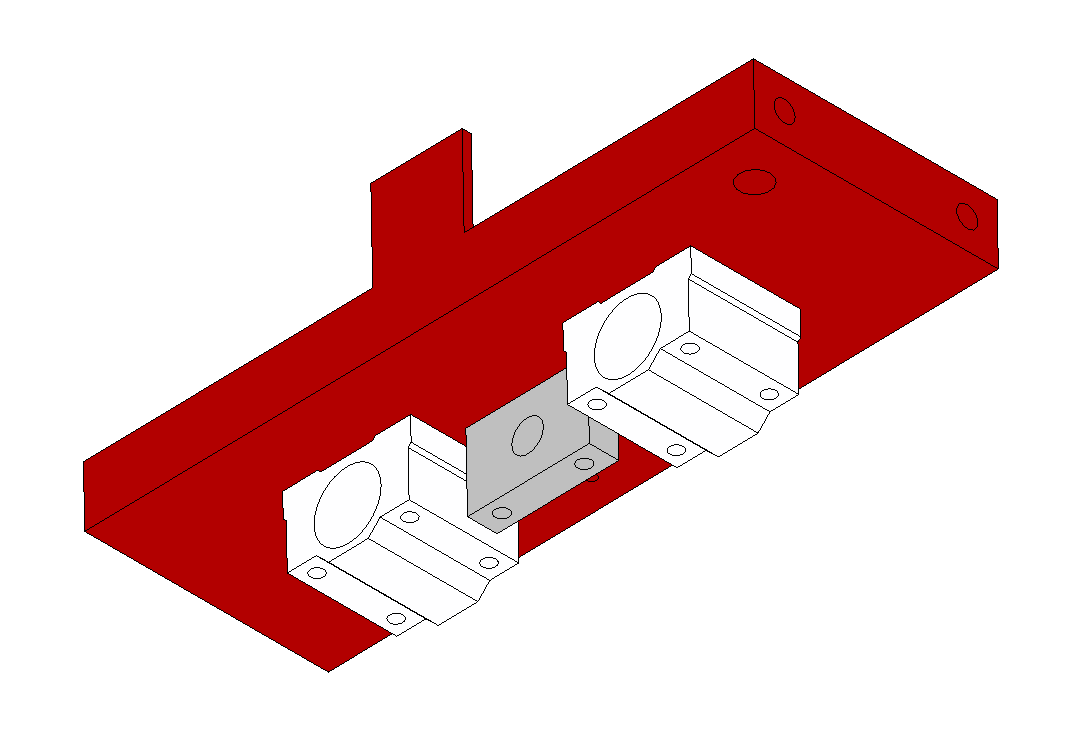
\includegraphics[width=0.5\textwidth]{images/x_axis/step_B.png}
        \caption{Assembly of the \textit{universal mount} with two (2) SC12UU bearings and one (1) T8 nut housing.}
        \label{fig:xa_step_2}
    \end{figure}
    
    \item Attach the two (2) twelve (12) millimeter linear rods to the SHF12 linear rod supports. Use the provided M4 screw in the support. Attach the eight (8) millimeter lead screw to the KFL08 bearing. Secure the lead screw with the M2 screws on the bearing. The assembly is shown on figure \ref{fig:xa_step_3}
    
    \begin{figure}[H]
        \centering
        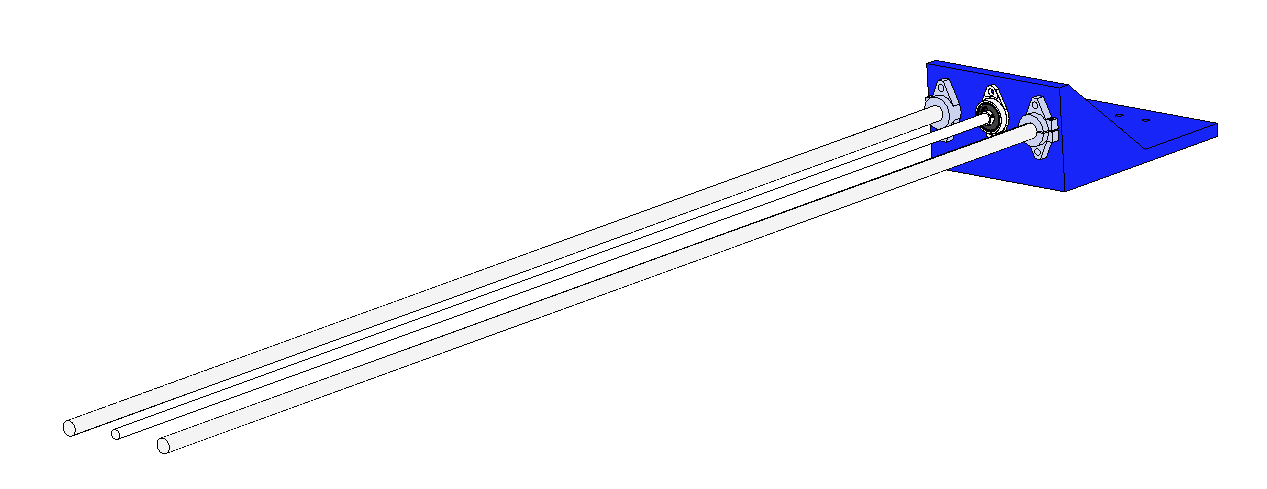
\includegraphics[width=0.9\textwidth]{images/x_axis/step_C.png}
        \caption{Assembly of the \textit{X-Axis auxiliary support} with the two (2) linear rods and the lead screw.}
        \label{fig:xa_step_3}
    \end{figure}
    
    \item Insert the \textit{universal mount} assembly in the linear rods and the lead screw. Keep the \textit{universal mount} assembly at the end of the linear rods to avoid damaging the assembly. Rotate the screw to adjust the position of the universal mount. The X-Axis assembly is shown on figure \ref{fig:xa_step_4}.
    
    \begin{figure}[H]
        \centering
        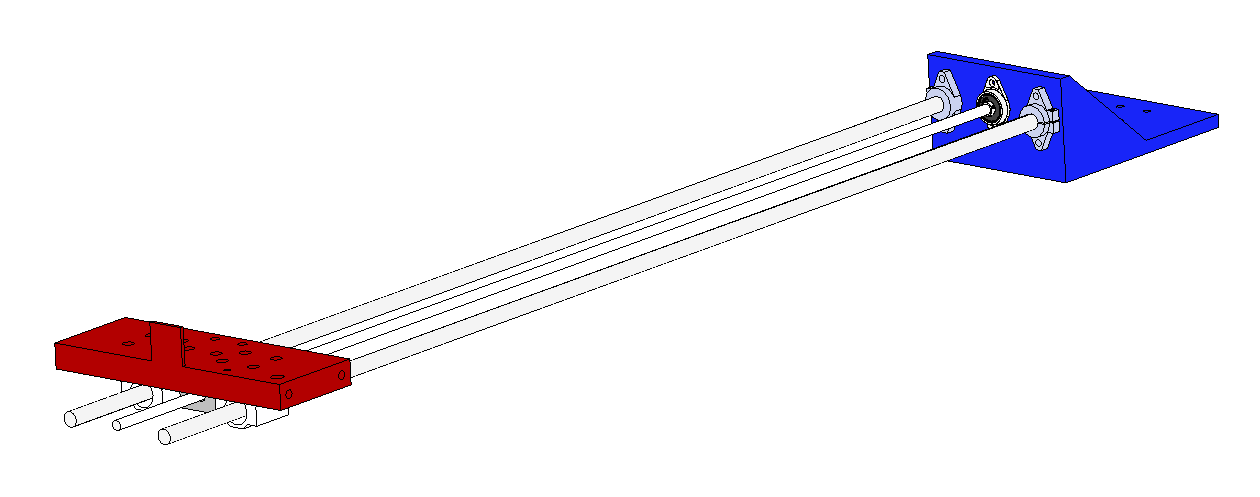
\includegraphics[width=0.9\textwidth]{images/x_axis/step_D.png}
        \caption{X-Axis assembly.}
        \label{fig:xa_step_4}
    \end{figure}

\end{enumerate}

\newpage
\section{VNA Holder Assembly}
\begin{enumerate}
    \item Focus on the \textit{side panel} of the VNA holder assembly. Consider both \textit{side panel} elements. You will notice four (4) holes in the top and bottom of each part. These holes are intended for M5 inserts. Using either a heat gun or a soldering iron, heat the inserts and place them into the holes. Allow the inserts to cool down. You will use the \textit{side panels} later in the assembly. The \textit{side panel} components are shown on figure \ref{fig:vna_holder_1}.
    
    \begin{figure}[H]
        \centering
        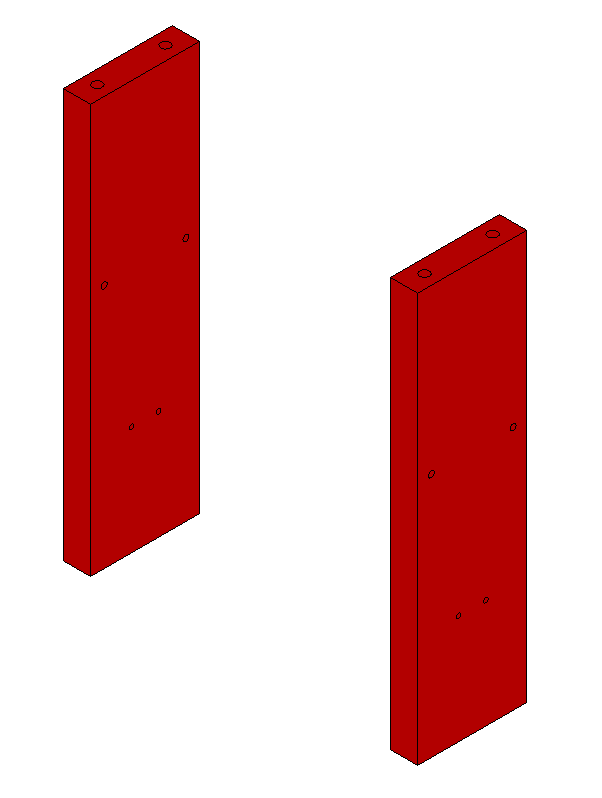
\includegraphics[width=0.3\textwidth]{images/vna_holder/step_A.png}
        \caption{\textit{Side panel} of the VNA holder assembly.}
        \label{fig:vna_holder_1}
    \end{figure}
    
    \item Take the \textit{antennae mount} element. Notice the slots for two NEMA17 stepper motors. The stepper motors are secured in place using four (4) M3 screws. Secure the stepper motors with the screws and make sure that the motor cables are located in the right side. The \textit{antennae mount} element is shown in figure \ref{fig:vna_holder_2}.
    
    \begin{figure}[H]
        \centering
        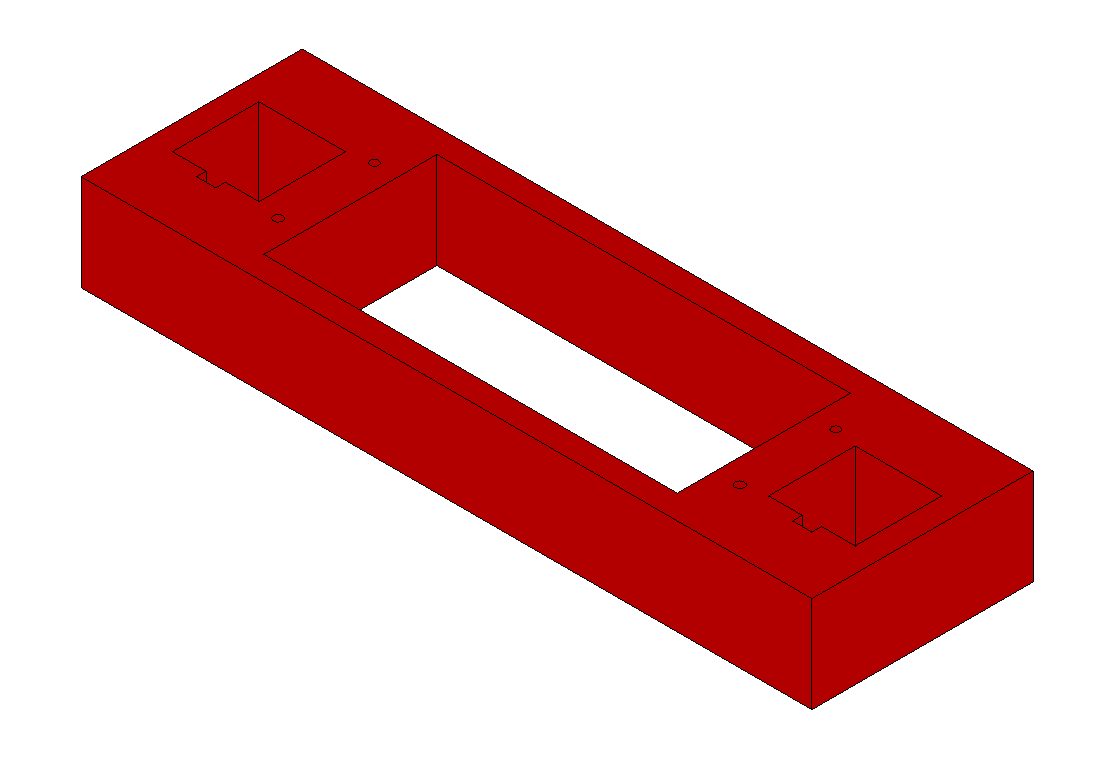
\includegraphics[width=0.4\textwidth]{images/vna_holder/step_B.png}
        \caption{\textit{Antennae mount} of the VNA holder assembly.}
        \label{fig:vna_holder_2}
    \end{figure}
    
    \item Merge the \textit{side panels} the \textit{antennae mount} using four (4) M5 screws. The screws are inserted from the bottom of the \textit{antennae mount}. The result of the assembly is shown on figure \ref{fig:vna_holder_3}. Notice the orientation of the holes in the \textit{side panel} components i.e. the position of the wide and narrow holes, with the latter being at the bottom.
    
    \begin{figure}[H]
        \centering
        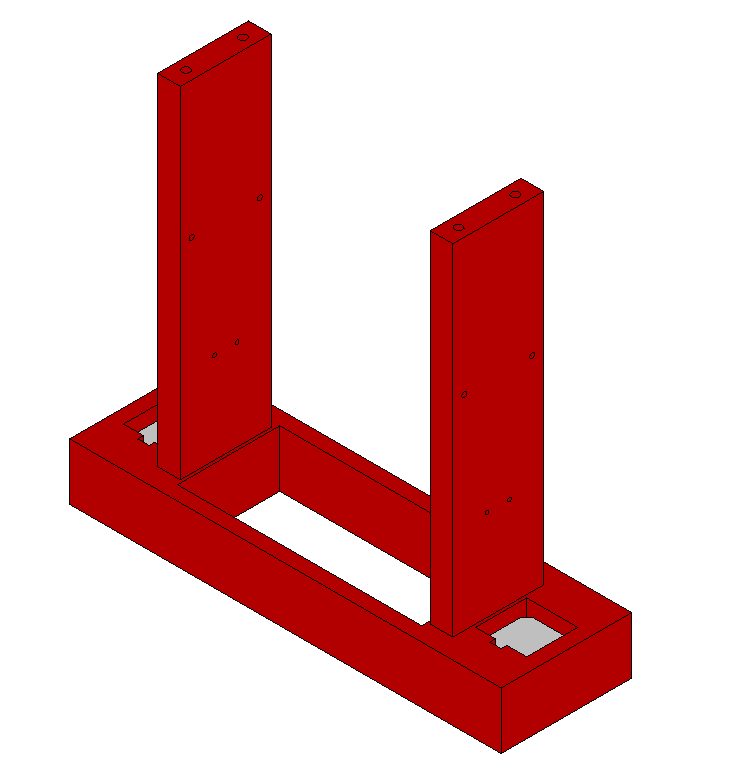
\includegraphics[width=0.4\textwidth]{images/vna_holder/step_C.png}
        \caption{\textit{Antennae mount} and the \textit{side panel} elements of the VNA holder assembly.}
        \label{fig:vna_holder_3}
    \end{figure}
    
    \item focus on the \textit{auxiliary strut}. The \textit{auxiliary strut} has four holes at its lateral sides. These holes are intended for M3 inserts. Heat four (4) M3 inserts using a heat gun or a soldering iron. Place the inserts into their respective holes. Allow the inserts to cool down before proceeding. Attach the \textit{auxiliary strut} to the \textit{side panel} elements using four (4) M3 screws. The assembly is shown on figure \ref{fig:vna_holder_4}.
    
    \begin{figure}[H]
        \centering
        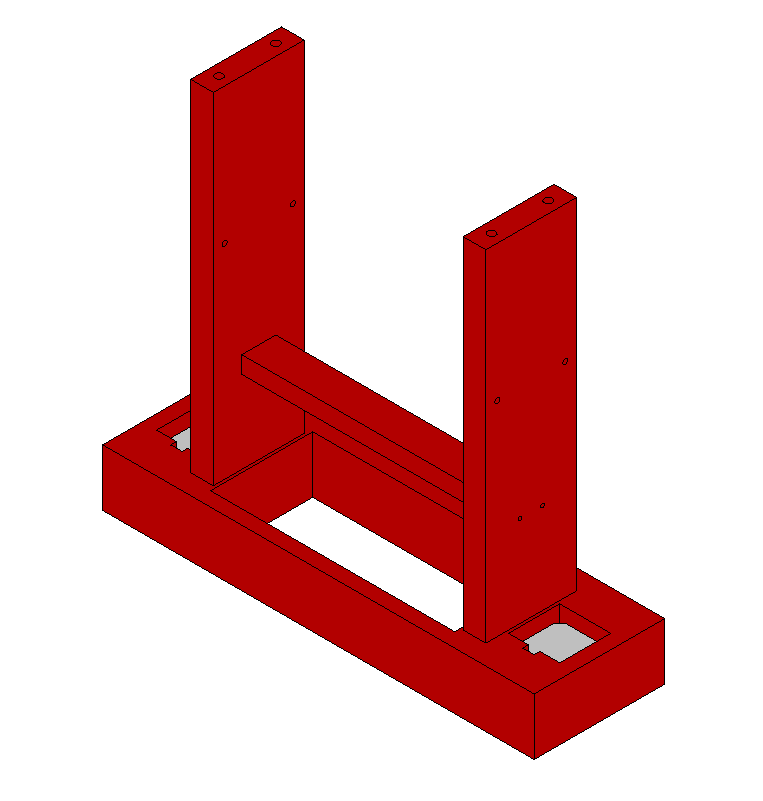
\includegraphics[width=0.4\textwidth]{images/vna_holder/step_D.png}
        \caption{\textit{Antennae mount}, \textit{auxiliary strut} and the \textit{side panel} elements of the VNA holder assembly.}
        \label{fig:vna_holder_4}
    \end{figure}
    
    \item Consider both the \textit{auxiliary axis support} and \textit{auxiliary axis cap}. Two items of each part are required for this step. The \textit{auxiliary axis cap} has two holes intended for M3 inserts. Using a heat gun or a soldering iron, heat four (4) M3 inserts and place them in the \textit{auxiliary axis cap} elements. Allow the inserts to cool down before proceeding. Locate the \textit{auxiliary axis cap} underneath the \textit{auxiliary strut}. Place the \textit{auxiliary axis support} on top of the \textit{auxiliary strut} and secure it in place with two (2) M3 screws. Figure \ref{fig:vna_holder_5} presents the assembly.
 
     \begin{figure}[H]
        \centering
        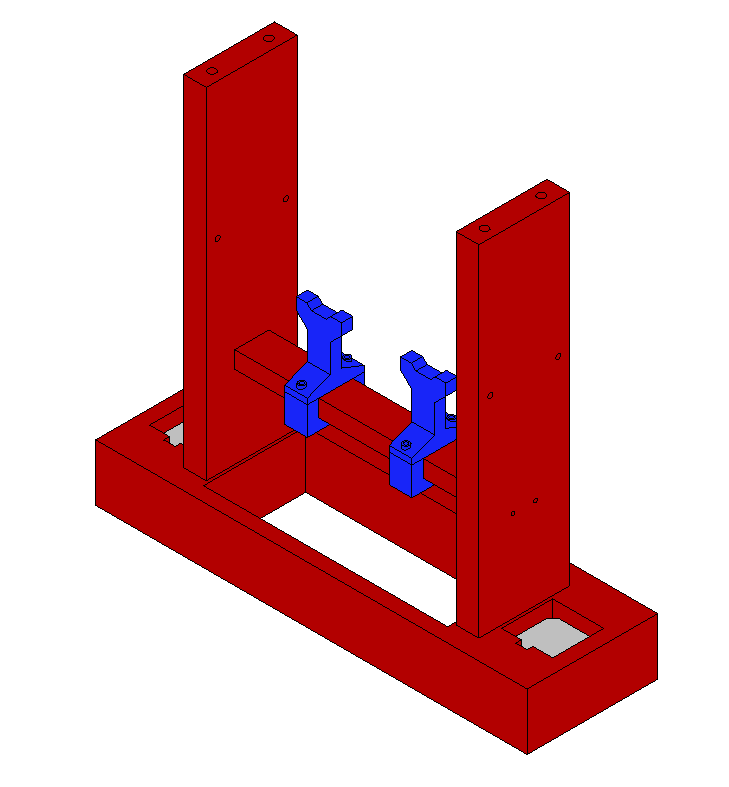
\includegraphics[width=0.35\textwidth]{images/vna_holder/step_E.png}
        \caption{GPR holder assembly with the \textit{auxiliary axis support} and \textit{auxiliary axis cap} elements attached.}
        \label{fig:vna_holder_5}
    \end{figure}
    
    \item Place the \textit{VNA mount} element on top of the assembly. Secure the part to the \textit{side panel} elements using four (4) M5 screws. The screws are attached from the top side of the \textit{VNA mount}. The assembly is shown on figure \ref{fig:vna_holder_6}.
    
    \begin{figure}[H]
        \centering
        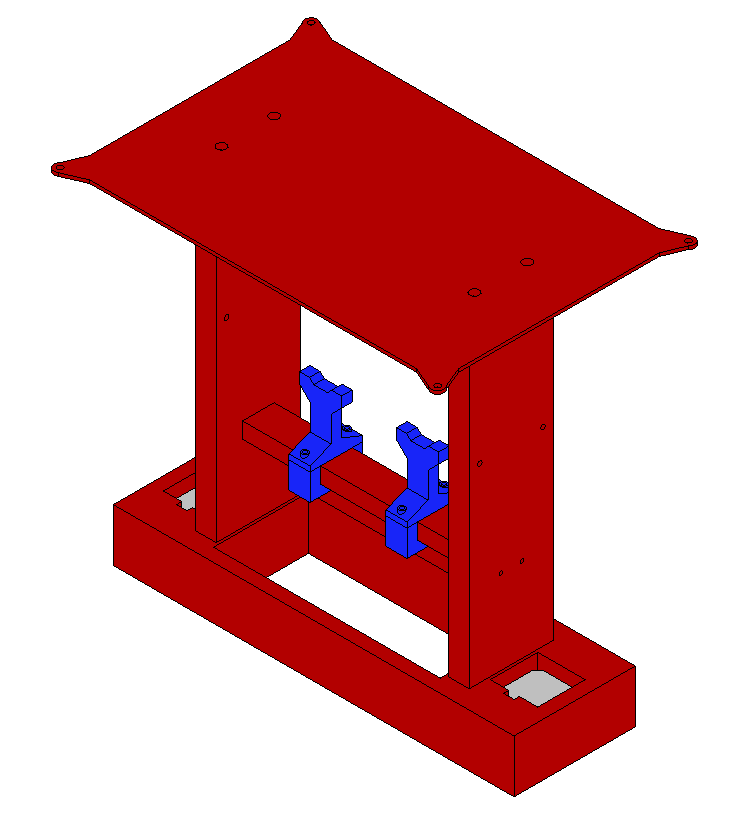
\includegraphics[width=0.35\textwidth]{images/vna_holder/step_F.png}
        \caption{GPR holder assembly with the \textit{VNA mount} attached on top.}
        \label{fig:vna_holder_6}
    \end{figure}
 
    \item Focus on the \textit{VNA cover} element. Notice the four holes at the bottom of the part. These holes are intended for M5 inserts. Heat four (4) M5 inserts using a heat gun or a soldering iron and place them into their respective holes. Allow the inserts to cool down. Attach the \textit{VNA cover} on top of the \textit{VNA mount} using four (4) M5 screws. Figure \ref{fig:vna_holder_7} shows the assembly.
    
    \begin{figure}[H]
        \centering
        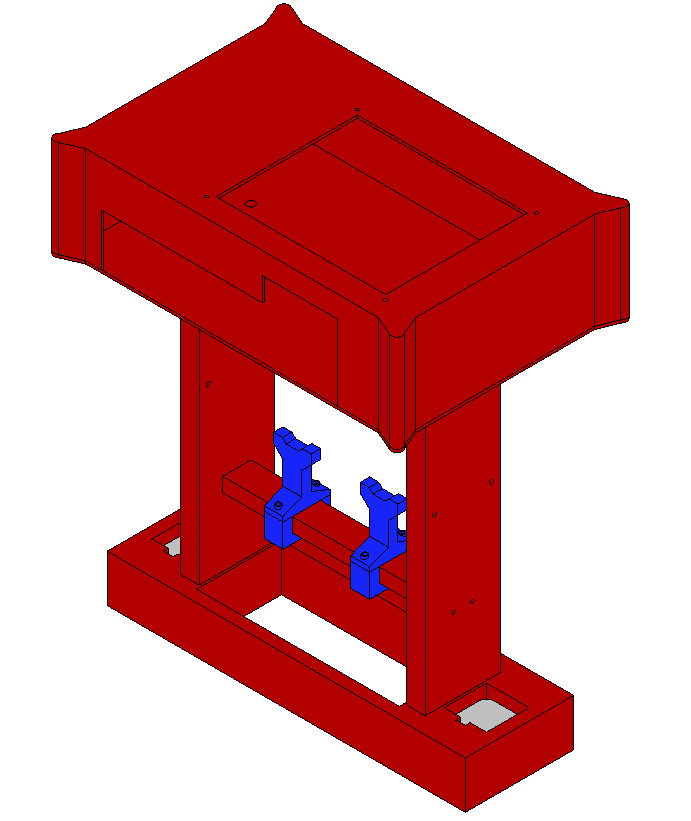
\includegraphics[width=0.35\textwidth]{images/vna_holder/step_G.png}
        \caption{GPR holder assembly with the \textit{VNA mount} attached on top.}
        \label{fig:vna_holder_7}
    \end{figure}
    
    \item Consider both the \textit{IR sensor support} and the \textit{IR sensor cap}. Identify the two holes for M3 inserts in the top side of the \textit{IR sensor support}. Heat two (2) M3 inserts with a heat gun or a soldering iron and place them into their respective holes. Allow the inserts to cool down before proceeding. Place the \textit{IR sensor support} underneath the central part of the \textit{antennae holder}. Secure the \textit{IR sensor support} in place with the \textit{IR sensor cap} using two (2) M3 screws. Attach the IR sensor using two (2) additional M3 screws. Figure \ref{fig:vna_holder_8} shows the assembly of the IR sensor mount.
    
    \begin{figure}[H]
        \centering
        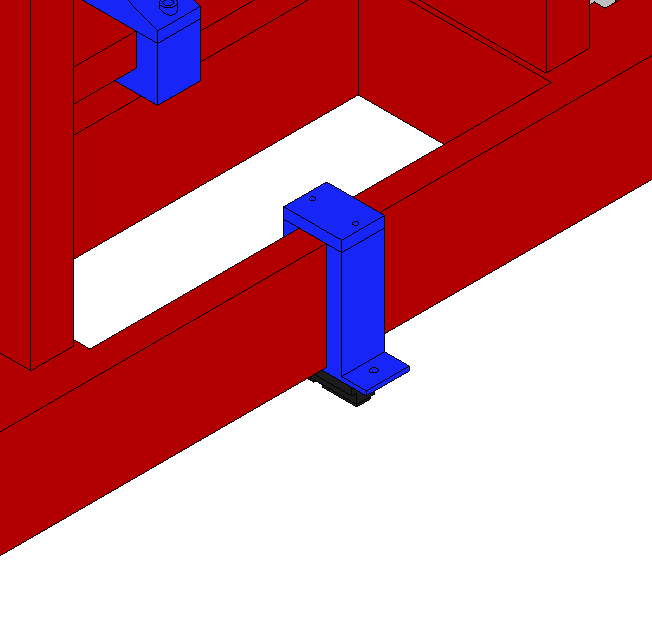
\includegraphics[width=0.35\textwidth]{images/vna_holder/step_H.png}
        \caption{GPR holder assembly with the \textit{VNA mount} attached on top.}
        \label{fig:vna_holder_8}
    \end{figure}
    
\end{enumerate}

\newpage
\section{Electronics Box Assembly}
\begin{enumerate}
    
    \item Take the \textit{power supply case} of the electronics box. Attach the Meanwell power supply with four M3 screws. The power supply holes are located from the bottom of the \textit{power supply case}. Connect the cables for the power supply. The cables are: a power cord to the power supply input, and three (2) couple of cables for the power supply output. Make sure to pass the power cord though the right hole of the case. Notice the holes in the upper side of the \textit{power supply case}. These holes are intended for M3 inserts. Heat four (4) M3 inserts with either a heat gun or a soldering iron and place them into the holes. Allow for the inserts to cool down. The assembly is shown on figure \ref{fig:electronics_1}.
    
    \begin{figure}[H]
        \centering
        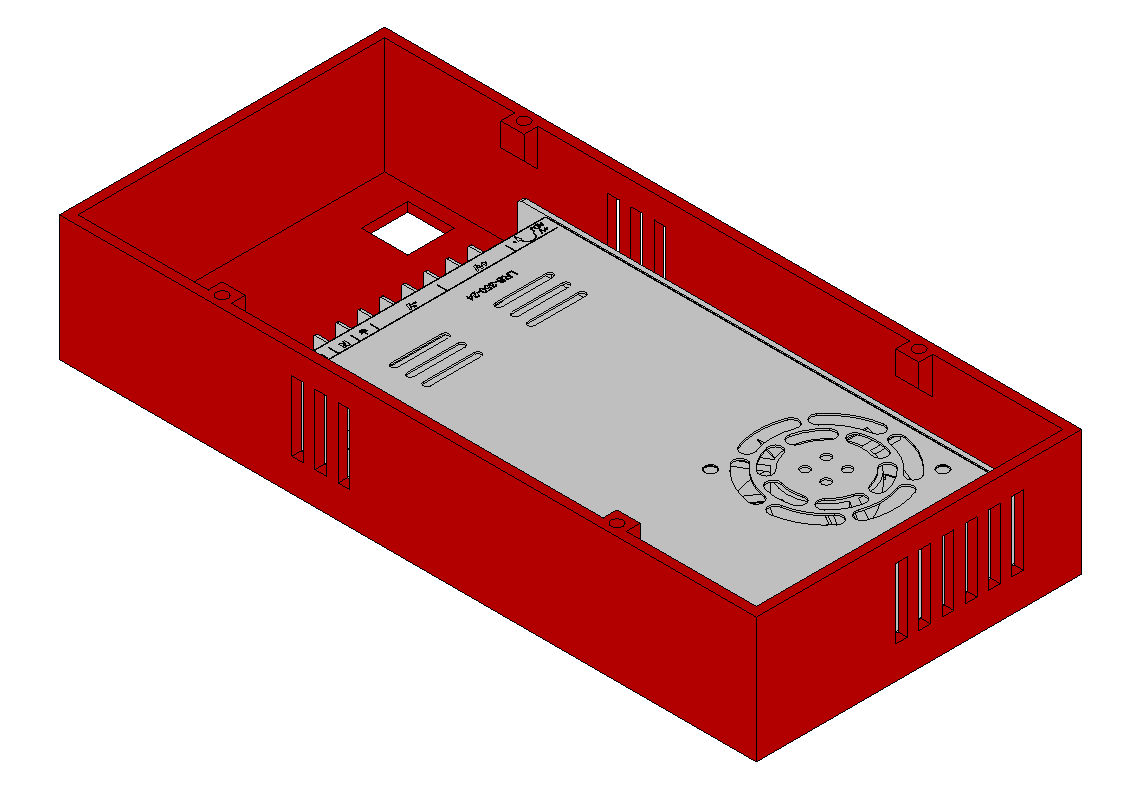
\includegraphics[width=0.5\textwidth]{images/electronics/step_A.png}
        \caption{\textit{Power supply case} with the power supply mounted.}
        \label{fig:electronics_1}
    \end{figure}
    
    \item Attach the \textit{lower PVC adapter} to the top of the \textit{power supply case}. Use four (4) M3 screws for this process. Identify the holes in the top side of the part. These holes are used to hold four (4) M4 inserts. Place the M4 inserts into the holes after heating them. Allow for the inserts to cool down. The assembly is shown on figure \ref{fig:electronics_2}.
    
    \begin{figure}[H]
        \centering
        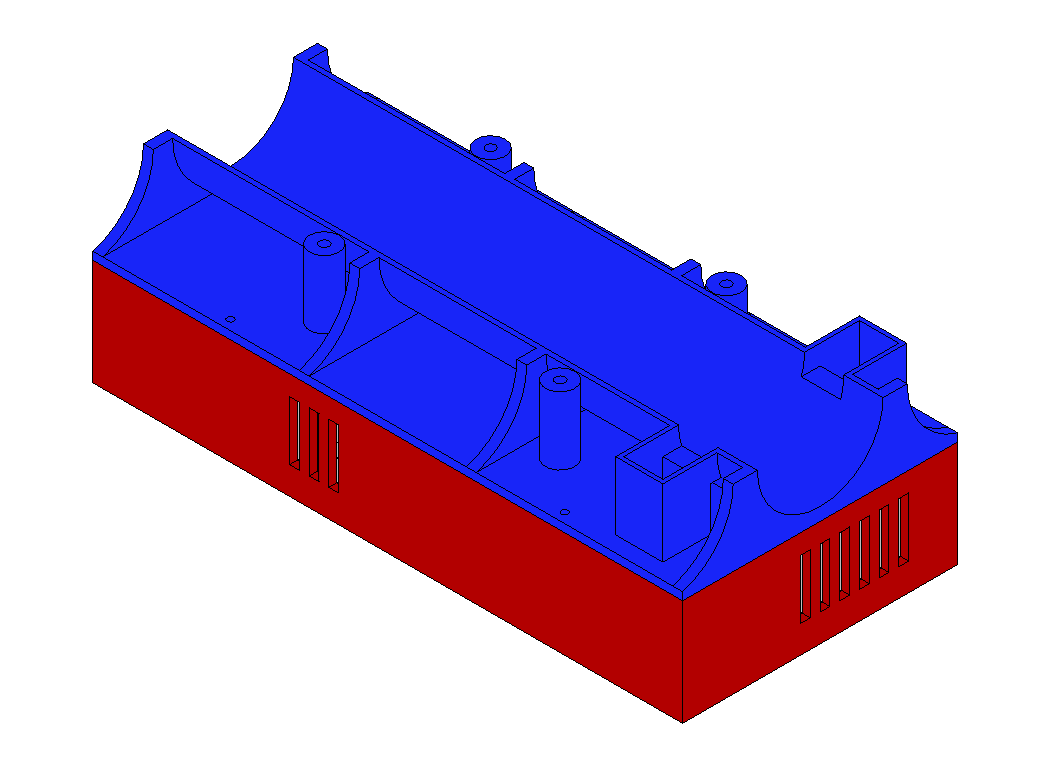
\includegraphics[width=0.5\textwidth]{images/electronics/step_B.png}
        \caption{\textit{Lower PVC adapter} mounted on top of the \textit{power supply case}.}
        \label{fig:electronics_2}
    \end{figure}
    
    \item Attach the \textit{upper PVC adapter} on top of the \textit{lower PVC adapter}. Use four M4 screws for this process. Leave the assembly aside once finished. The result of the assembly is shown on figure \ref{fig:electronics_3}.
    
    \begin{figure}[H]
        \centering
        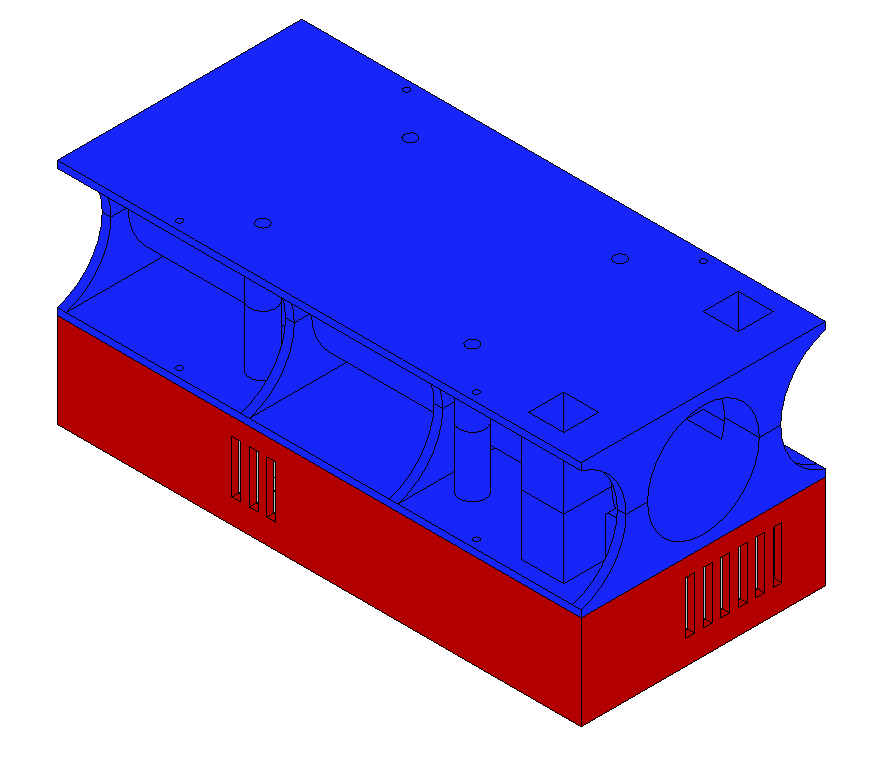
\includegraphics[width=0.5\textwidth]{images/electronics/step_C.png}
        \caption{\textit{Upper PVC adapter} attached on top of the \textit{lower PVC adapter}.}
        \label{fig:electronics_3}
    \end{figure}
    
    \item Attach the touchscreen to the \textit{touchscreen lid} using four (4) M3 screws with their corresponding nuts. Leave the assembly aside once finished. The touchscreen and the \textit{touchscreen lid} element assembly is shown on figure \ref{fig:electronics_4}.
    
    \begin{figure}[H]
        \centering
        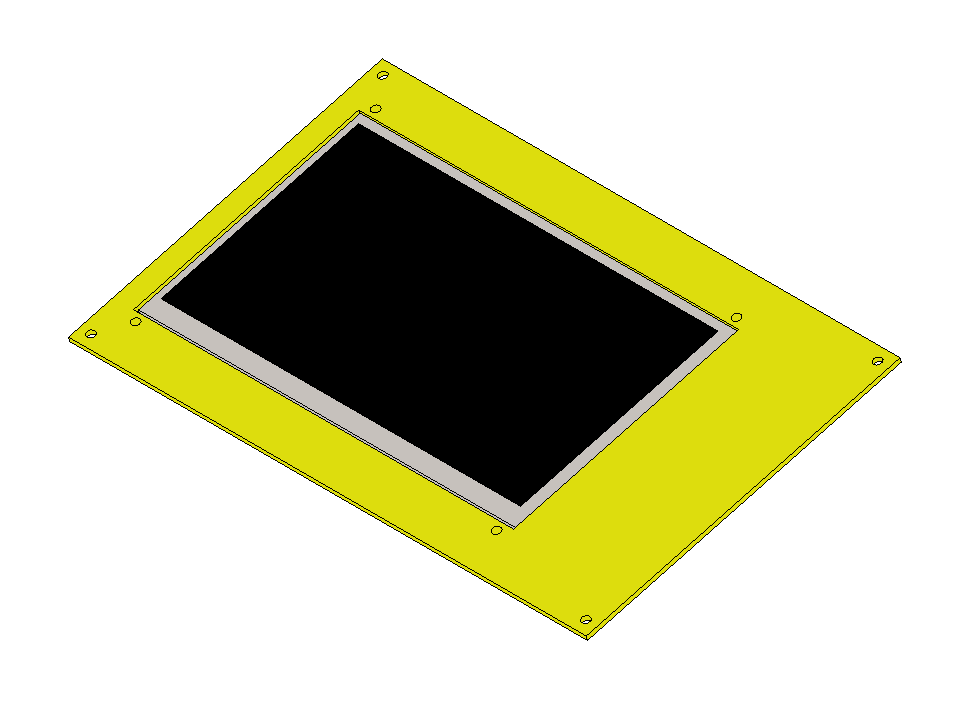
\includegraphics[width=0.5\textwidth]{images/electronics/step_D.png}
        \caption{Touchscreen and \textit{touchscreen lid} assembly.}
        \label{fig:electronics_4}
    \end{figure}
    
    \item Identify the bottom holes of the \textit{electronics case}. These holes are intended for M3 inserts. Heat four (4) M3 using either a heat gun or a soldering iron. Place the heated inserts in their corresponding holes. Allow the inserts to cool down. Identify the four (4) holes in the lateral and opened side of the \textit{electronics case}. These holes are intended for M3 inserts. Heat the M3 inserts and place them into the corresponding holes. Identify the four (4) holes in the angled face of the \textit{touchscreen support}. These holes are intended for M3 inserts. Heat the M3 inserts and place them into the corresponding holes. Allow the inserts to cool down. Attach the \textit{touchscreen support} to the \textit{electronics case}. Use four (4) M3 screws with their corresponding nuts. The assembly is shown on figure \ref{fig:electronics_5}.
    
    \begin{figure}[H]
        \centering
        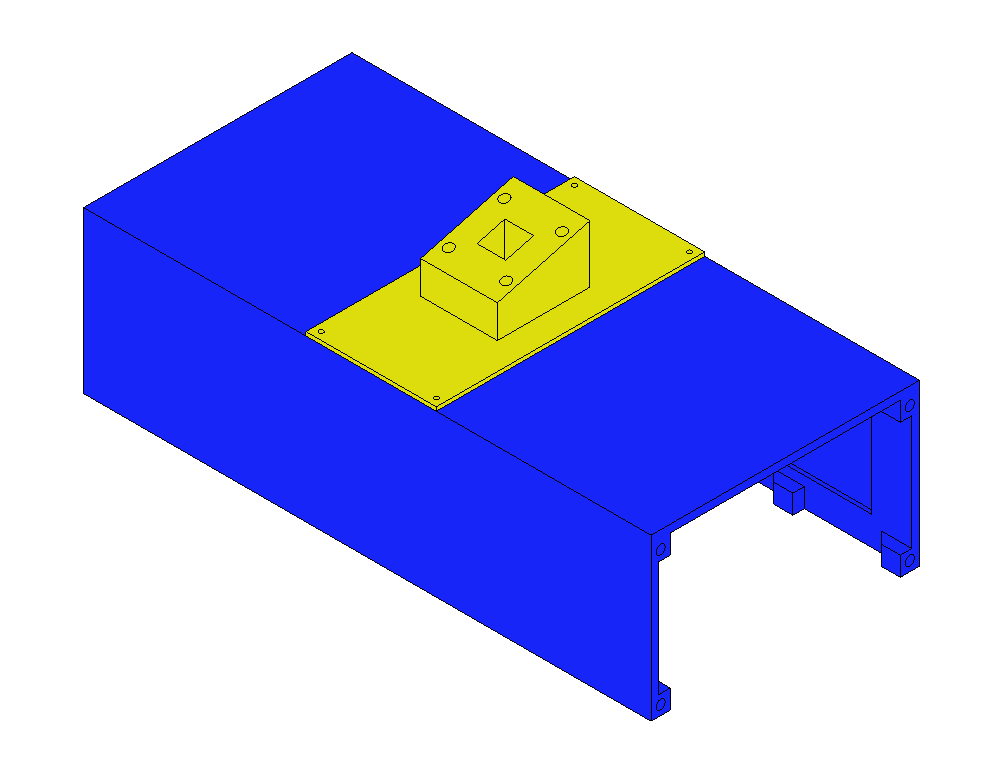
\includegraphics[width=0.5\textwidth]{images/electronics/step_E.png}
        \caption{\textit{Electronics case} and \textit{touchscreen support} assembly.}
        \label{fig:electronics_5}
    \end{figure}
    
    \item Identify the four (4) holes on the top face of the \textit{touchscreen case} element. These holes are intended for M3 inserts. Heat the four (4) M3 inserts with either a heat gun or a soldering iron. Place the heated inserts in the aforementioned holes. Allow for the inserts to cool down before proceeding. Attach the \textit{touchscreen case} to the angled face of the \textit{touchscreen support} using four (4) M3 screws. The assembly is shown on figure \ref{fig:electronics_6}.
    
    \begin{figure}[H]
        \centering
        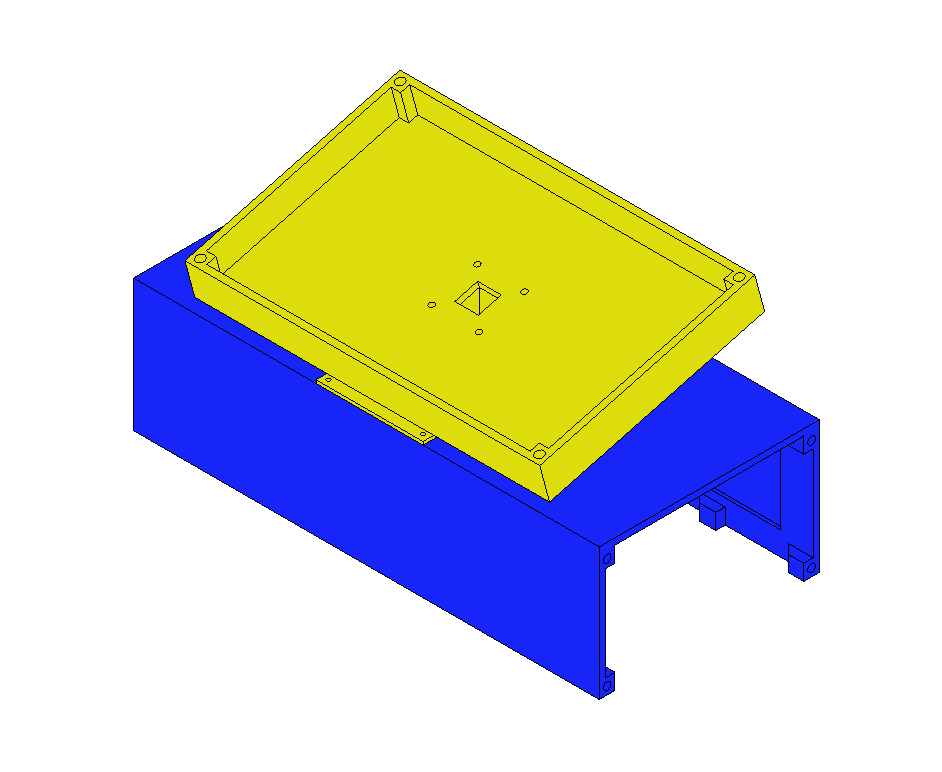
\includegraphics[width=0.5\textwidth]{images/electronics/step_F.png}
        \caption{\textit{Touchscreen case} attached to the \textit{touchscreen support}.}
        \label{fig:electronics_6}
    \end{figure}
    
    \item Connect the USB power and HDMI cables into the touchscreen. Pass the cables trough the center hole of the \textit{touchscreen case} until it comes out inside the \textit{electronics case}. Attach the \textit{touchscreen lid} to the \textit{touchscreen case} using four (4) M3 screws. The result of the assembly is shown on figure \ref{fig:electronics_7}.
    
    \begin{figure}[H]
        \centering
        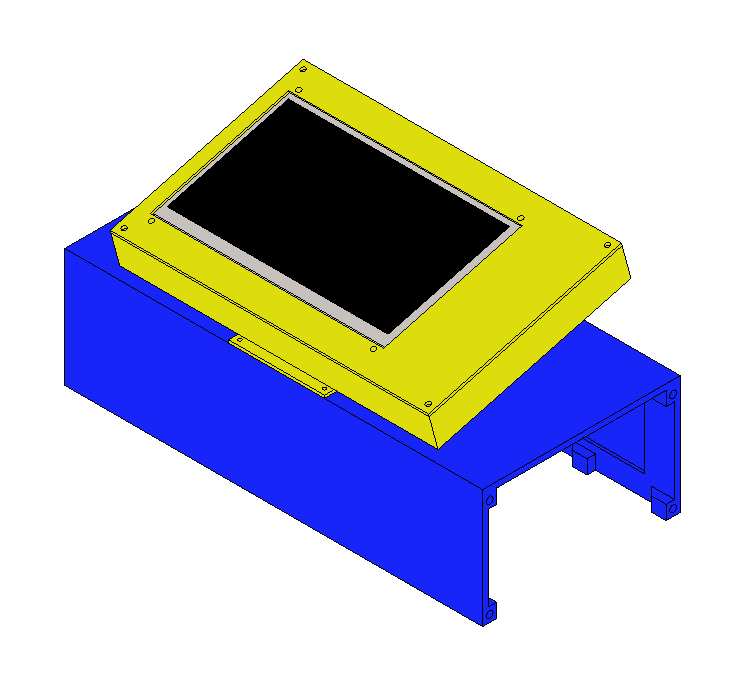
\includegraphics[width=0.5\textwidth]{images/electronics/step_G.png}
        \caption{\textit{Touchscreen lid} attached to the \textit{electronics case} assembly.}
        \label{fig:electronics_7}
    \end{figure}
    
    \item Identify the \textit{electronics board tray} and the \textit{Raspi board tray}. Both board trays have holes on their top surface that are intended for M2 and M3 inserts. The \textit{electronics board tray} has two (2) holes for M3 inserts. Place the two (2) M3 inserts in the tray after heating them up. Allow for the inserts to cool down before proceeding. The \textit{Raspi board tray} has twelve (12) holes for M2 inserts. Place the inserts into their corresponding holes after heating them up. Allow for the inserts to cool down before proceeding. The \textit{Rasspi board tray} has four (4) additional holes on top of the column-like supports of the board. These holes use M2 inserts. Place the four (4) M2 inserts in the holes at the supports. Attach the electronics to the board trays using M2 screws. Make sure to have soldered the required cables and connectors to the components before attaching them to the trays. Place the \textit{electronics board tray} on top of the \textit{Raspi board tray} and attach the latter with four (4) M2 screws. Locate the holes at the lateral parts of the trays and place eighth (8) M2 heated inserts into them. Allow the inserts to cool down. Insert the trays into the \textit{electronics case} and secure them with four (4) M2 screws. It must be noted that the electronics connections of the boards will be addressed in the field setup. The assembly is shown on figure \ref{fig:electronics_8}.
    
    \begin{figure}[H]
        \centering
        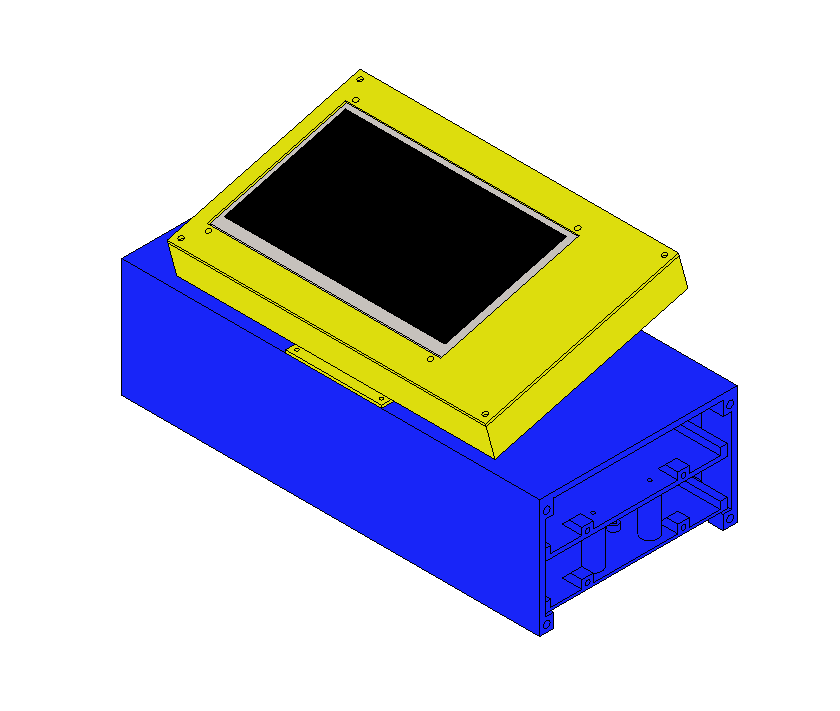
\includegraphics[width=0.5\textwidth]{images/electronics/step_H.png}
        \caption{\textit{Electronics case} with the trays secured in place.}
        \label{fig:electronics_8}
    \end{figure}
    
    \item Attach the \textit{electronics case panel} to the \textit{electronics case} using four (4) M3 screws. Secure the \textit{electronics case panel} to the board trays using four (4) M2 screws. The assembly is shown on figure \ref{fig:electronics_9}. 
    
    \begin{figure}[H]
        \centering
        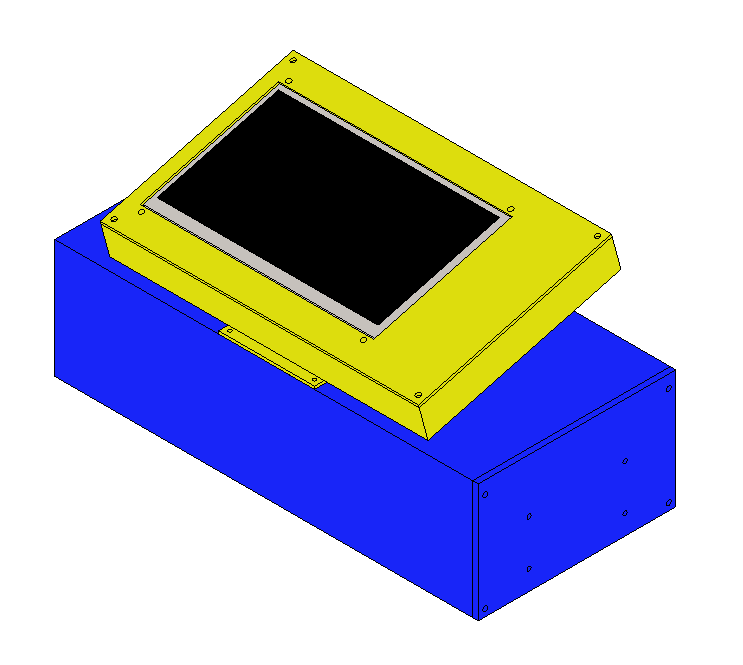
\includegraphics[width=0.5\textwidth]{images/electronics/step_I.png}
        \caption{\textit{Electronics case panel} attached to the \textit{electronics case}.}
        \label{fig:electronics_9}
    \end{figure}
    
    \item Attach the \textit{electronics case} to the \textit{upper PVC adapter}. Use four (4) M3 screws for this process. The assembly is shown on figure \ref{fig:electronics_10}.
    
    \begin{figure}[H]
        \centering
        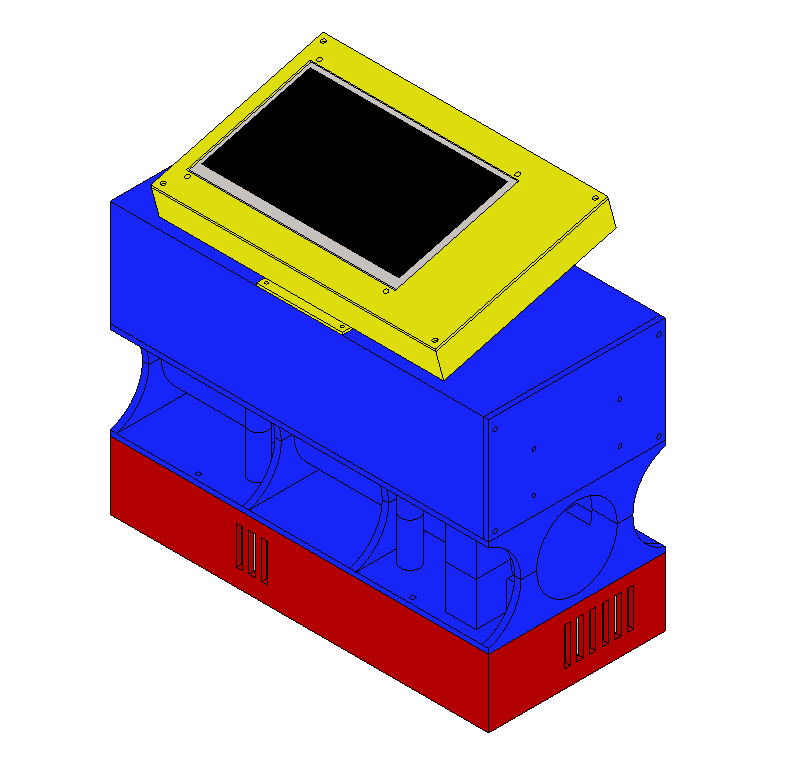
\includegraphics[width=0.5\textwidth]{images/electronics/step_J.png}
        \caption{\textit{Electronics case} attached on top of the \textit{upper PVC adapter}.}
        \label{fig:electronics_10}
    \end{figure}
    
    \item Pass a one meter long PVC tube into the \textit{upper and lower PVC adapters}. The fully electronics box is assembled in figure \ref{fig:electronics_11}.
    
    \begin{figure}[H]
        \centering
        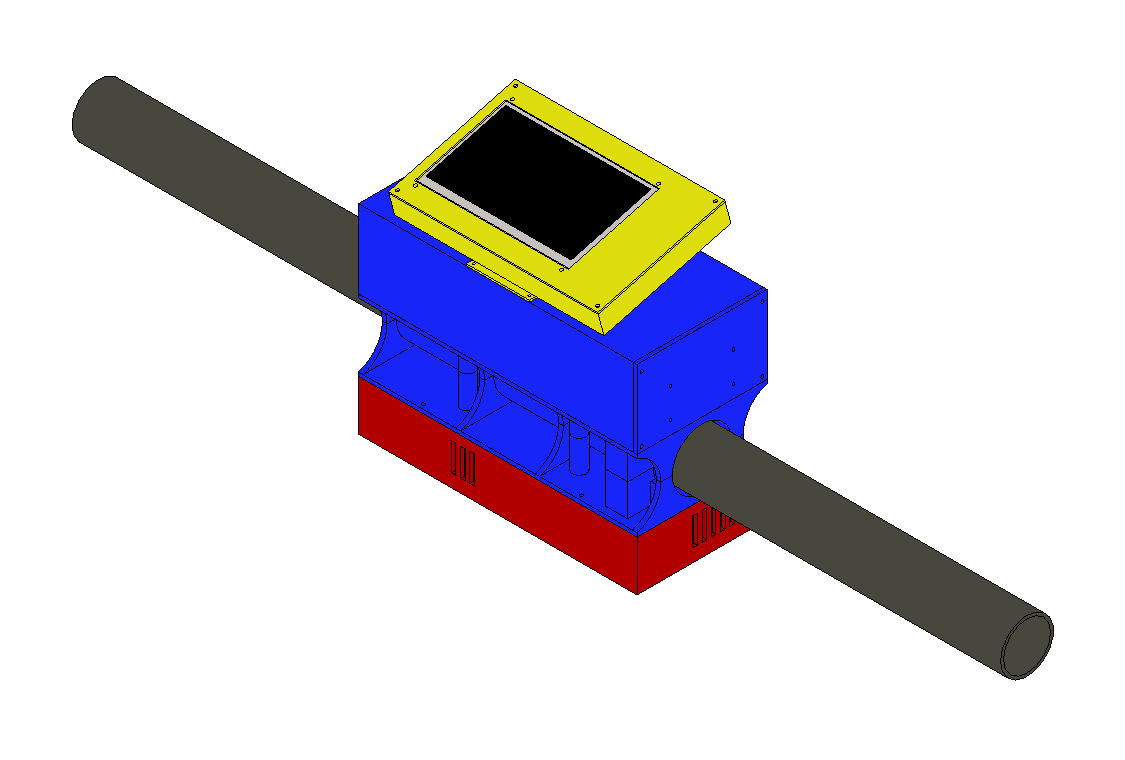
\includegraphics[width=0.5\textwidth]{images/electronics/step_K.png}
        \caption{Electronics box fully assembled.}
        \label{fig:electronics_11}
    \end{figure}
    
\end{enumerate}

\newpage
\section{Robot Cabling}
This section presents the process of cabling the robot. The section is divided depending on the device that will be cabled. Follow each section before proceeding to the field setup manual. 

\subsection{Antennae Motors}
\begin{figure}[H]
    \centering
    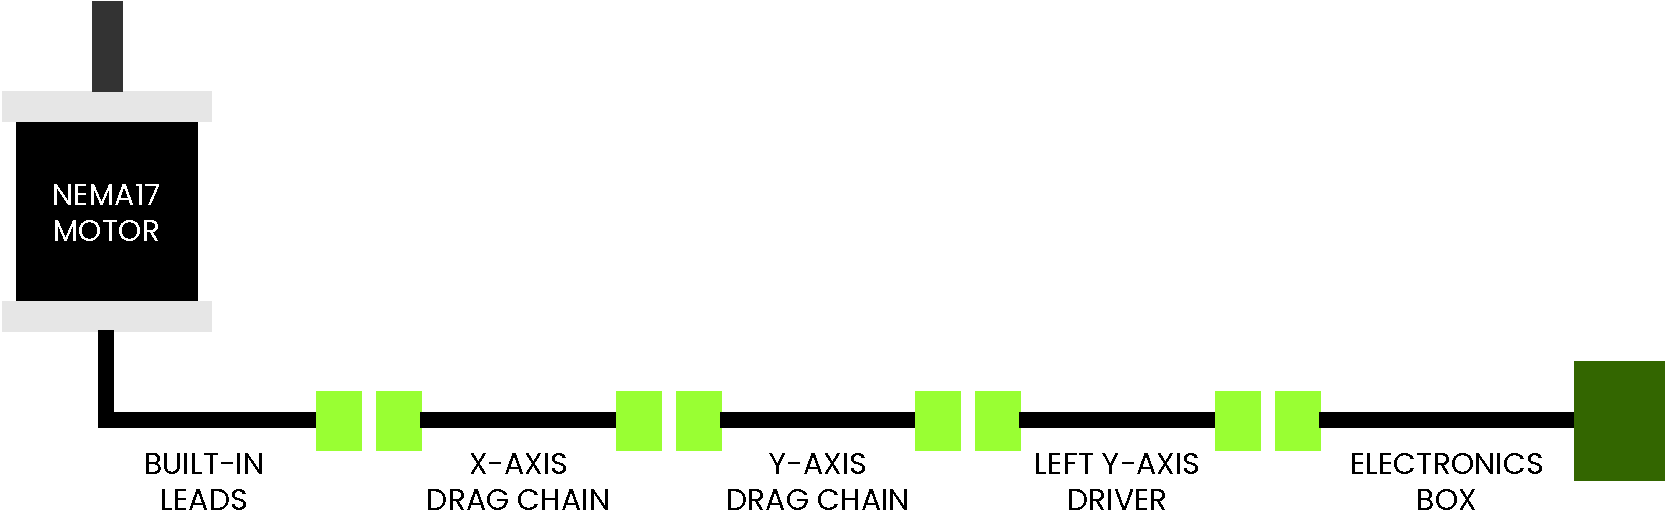
\includegraphics[width=0.8\textwidth]{images/cabling/NEMA17_antennae.pdf}
    \caption{Cabling stages for the antennae motors.}
    \label{fig:cabling_antennae_motors}
\end{figure}
The cabling for the antennae motors consists of providing them with power from the electronics board to the motors themselves. The cabling should be done in such a way that its parts are located in the different major components. Figure \ref{fig:cabling_antennae_motors} presents the cabling stages for the antennae motors. A total of eight (8) 4-pin connectors and 4350 millimeters of 4-phases cable are needed in order to execute the antennae motors cabling. Table \ref{tab:cabling_antennae_motors} presents the procedure for cabling the antennae motors.

\begin{singlespace}
\begin{xltabular}{\textwidth}{|c|X|}
    
    \hline \multicolumn{2}{|c|}{\textbf{Antennae motors cabling}} \\ \hline
    \endhead
    
    \hline \multicolumn{2}{|c|}{\textbf{Antennae motors cabling}} \\ \hline
    \endfirsthead
    
    \multicolumn{2}{|c|}{\textit{Continues on next page.}} \\ \hline
    \endfoot
    
    \caption{Antennae motor cabling process.} \label{tab:cabling_antennae_motors}
    \endlastfoot
    
    $\square$ & Peel the motors built-in cable tips. Solder or join the cable tips to the female side of one connector. Isolate the connections to prevent short-circuiting the motor phases. Repeat the process for both motors. \\ \hline
    $\square$ & Measure the distance between the motor connectors and the X-Axis driver support through the X-Axis drag chain. This will be distance of the motor cables from the GPR to the X-Axis driver. Make sure that cables are not under tension. Cut a piece of cable with the proper length. \\ \hline
    $\square$ & Pass the cable through the X-Axis drag chain. Peel the X-Axis cable tips and solder them to a male and female connector. The male connector will be used in the GPR side of the X-Axis drag chain. Keep in mind that the drag chain sides are not interchangeable. \\ \hline
    $\square$ & Measure the distance from the cable tip at the X-Axis driver support and the left Y-Axis driver trough the drag chain. This will be the cable distance from the X-Axis driver and the left Y-Axis driver. Remember to measure the distance through the drag chain. Cut a piece of cable with the proper length. \\ \hline
    $\square$ & Pass the cable through the Y-Axis drag chain. Peel the Y-Axis cable tips and solder them to a male and female connector. The male connector will be used in the X-Axis driver side of the Y-Axis drag chain. Keep in mind that the drag chains are not interchangeable. \\ \hline
    $\square$ & Measure the distance from the cable tip at the left Y-Axis driver support and the cable opening at support right side. You can use an auxiliary cable to measure that distance. Make sure to use the cable opening from the upper side of the support. Cut a piece of cable with the proper length. \\ \hline
    $\square$ & Pass the cable through the opening at the top of the left Y-Axis support. Peel the cable tips and solder a male and female connector at the tips. The male connector should be used to connect the cables at the end of the Y-Axis drag chain. \\ \hline
    $\square$ & Measure the distance between the cable opening at the side of the left Y-Axis driver and the electronics board. Measure the distance through the PVC tube and the cable opening of the electronics box. Cut a piece of cable with the proper length. \\ \hline
    $\square$ & Peel the  electronics box cable tips. Pass the cable from the opening of the PVC tube until it reaches the electronics board inside the electronics box. Solder a male connector at the tip located in the PVC tube. Connect the other cable tip with the corresponding plug of the electronics board. \\ \hline
    $\square$ & Test the continuity of the cable from the electronics board plug to the male connector from the X-Axis drag chain. Make sure that all the connectors are plugged. \\ \hline 
\end{xltabular}
\end{singlespace}

\subsection{X-Axis Motor Cabling}
\begin{figure}[H]
    \centering
    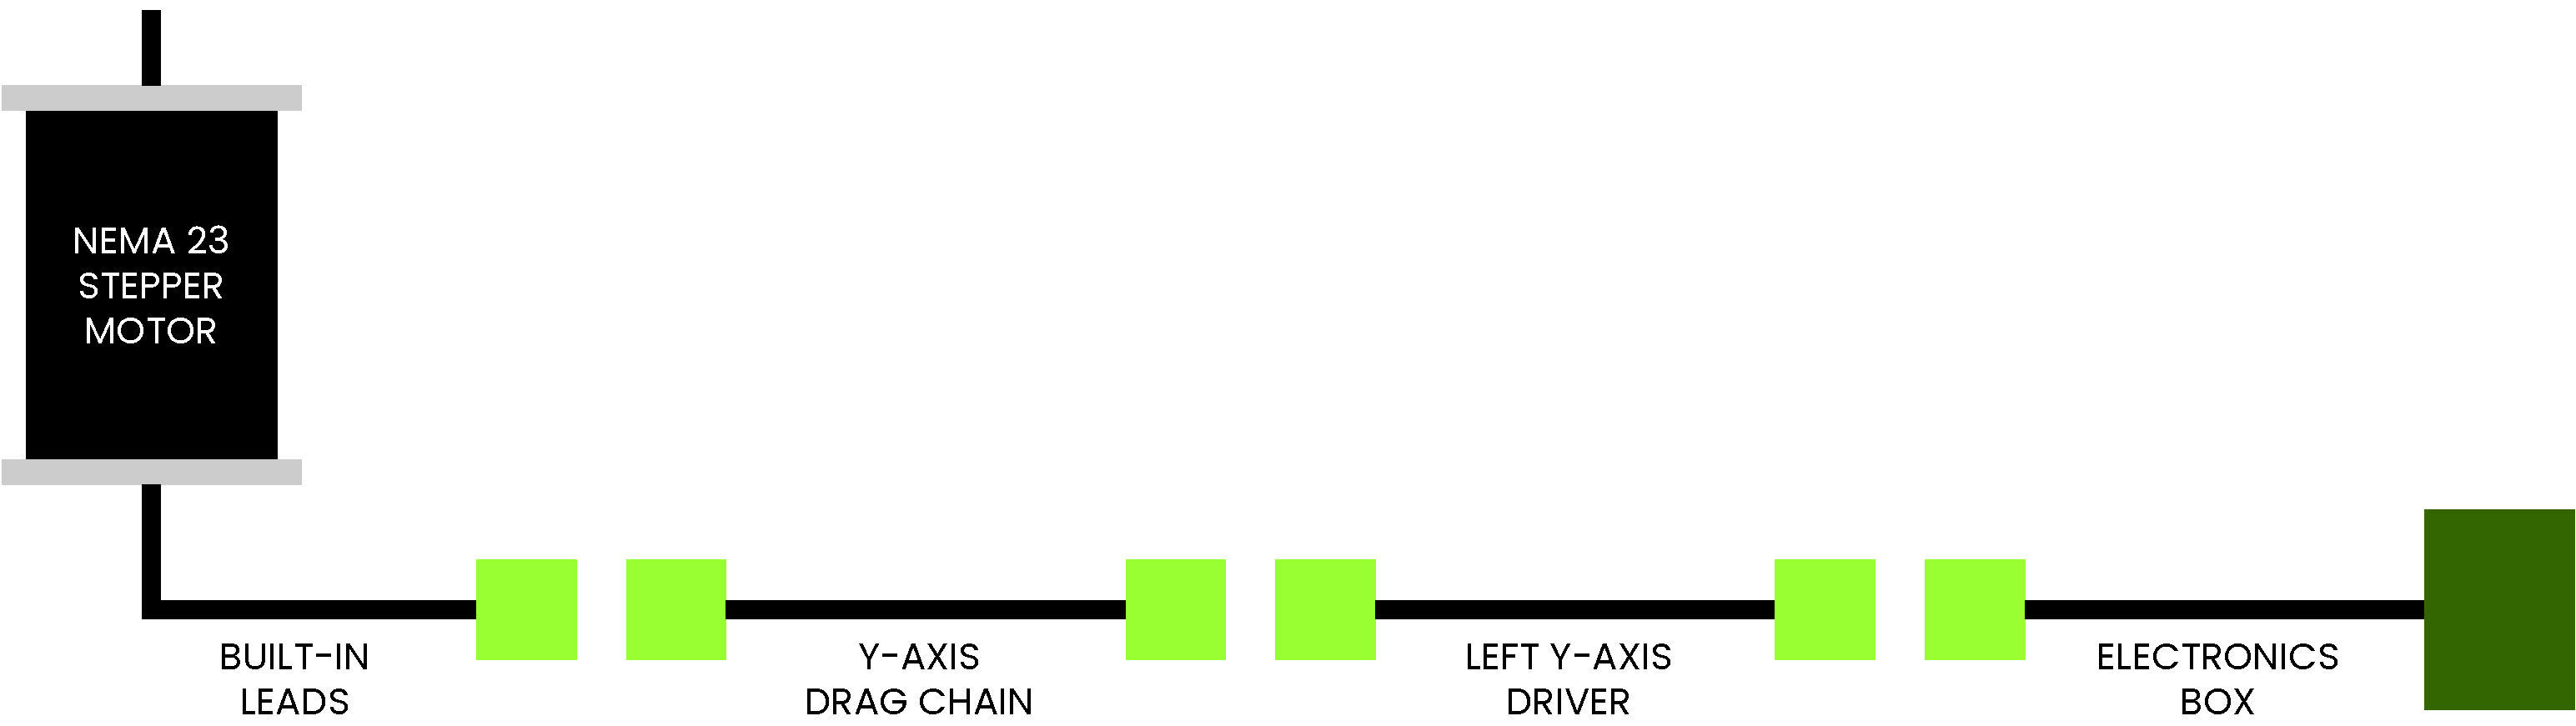
\includegraphics[width=0.8\textwidth]{images/cabling/x_axis_motors_cabling.pdf}
    \caption{Cabling stages for the X-Axis motor.}
    \label{fig:cabling_x_axis_motors}
\end{figure}
The cabling for the X-Axis motor consists of providing it with power from the electronics board to the motor itself. The cabling should be done in such a way that its parts are located in the different major components. Figure \ref{fig:cabling_x_axis_motors} presents the cabling stages for the X-Axis motor. A total of three (3) 4-pin connectors and 3250 millimeters of 4-phases cable are needed in order to execute the X-Axis motor cabling. Table \ref{tab:cabling_x_axis_motors} presents the procedure for cabling the X-Axis motor.

\begin{singlespace}
\begin{xltabular}{\textwidth}{|c|X|}
    
    \hline \multicolumn{2}{|c|}{\textbf{X-Axis motor cabling}} \\ \hline
    \endhead
    
    \hline \multicolumn{2}{|c|}{\textbf{X-Axis motor cabling}} \\ \hline
    \endfirsthead
    
    \multicolumn{2}{|c|}{\textit{Continues on next page.}} \\ \hline
    \endfoot
    
    \caption{X-Axis motor cabling process.} \label{tab:cabling_x_axis_motors}
    \endlastfoot
    
    $\square$ & Peel the motor built-in cable tips. Solder or join the cable tips to the female side of one connector. Isolate the connections to prevent short-circuiting the motor phases. \\ \hline
    $\square$ & Measure the distance between the motor connector and the left Y-Axis driver support through the Y-Axis drag chain. This will be distance of the motor cable from the X-Axis driver to the left Y-Axis driver. Make sure that cables are not under tension. Cut a piece of cable with the proper length. \\ \hline
    $\square$ & Pass the cable through the Y-Axis drag chain. Peel the Y-Axis cable tips and solder them to a male and female connector. The male connector will be used in the X-Axis driver side of the Y-Axis drag chain. Keep in mind that the drag chain sides are not interchangeable. \\ \hline
    $\square$ & Measure the distance from the cable tip at the left Y-Axis driver support and the cable opening at support right side. You can use an auxiliary cable to measure that distance. Make sure to use the cable opening from the upper side of the support. Cut a piece of cable with the proper length. \\ \hline
    $\square$ & Pass the cable through the opening at the top of the left Y-Axis support. Peel the cable tips and solder a male and female connector at the tips. The male connector should be used to connect the cables at the end of the Y-Axis drag chain. \\ \hline
    $\square$ & Measure the distance between the cable opening at the side of the left Y-Axis driver and the electronics board. Measure the distance through the PVC tube and the cable opening of the electronics box. Cut a piece of cable with the proper length. \\ \hline
    $\square$ & Peel the  electronics box cable tips. Pass the cable from the opening of the PVC tube until it reaches the electronics board inside the electronics box. Solder a male connector at the tip located in the PVC tube. Connect the other cable tip with the corresponding plug of the electronics board. \\ \hline
    $\square$ & Test the continuity of the cable from the electronics board plug to the male connector from the X-Axis drag chain. Make sure that all the connectors are plugged. \\ \hline 
\end{xltabular}
\end{singlespace}

\subsection{Y-Axis Motors}
\begin{figure}[H]
    \centering
    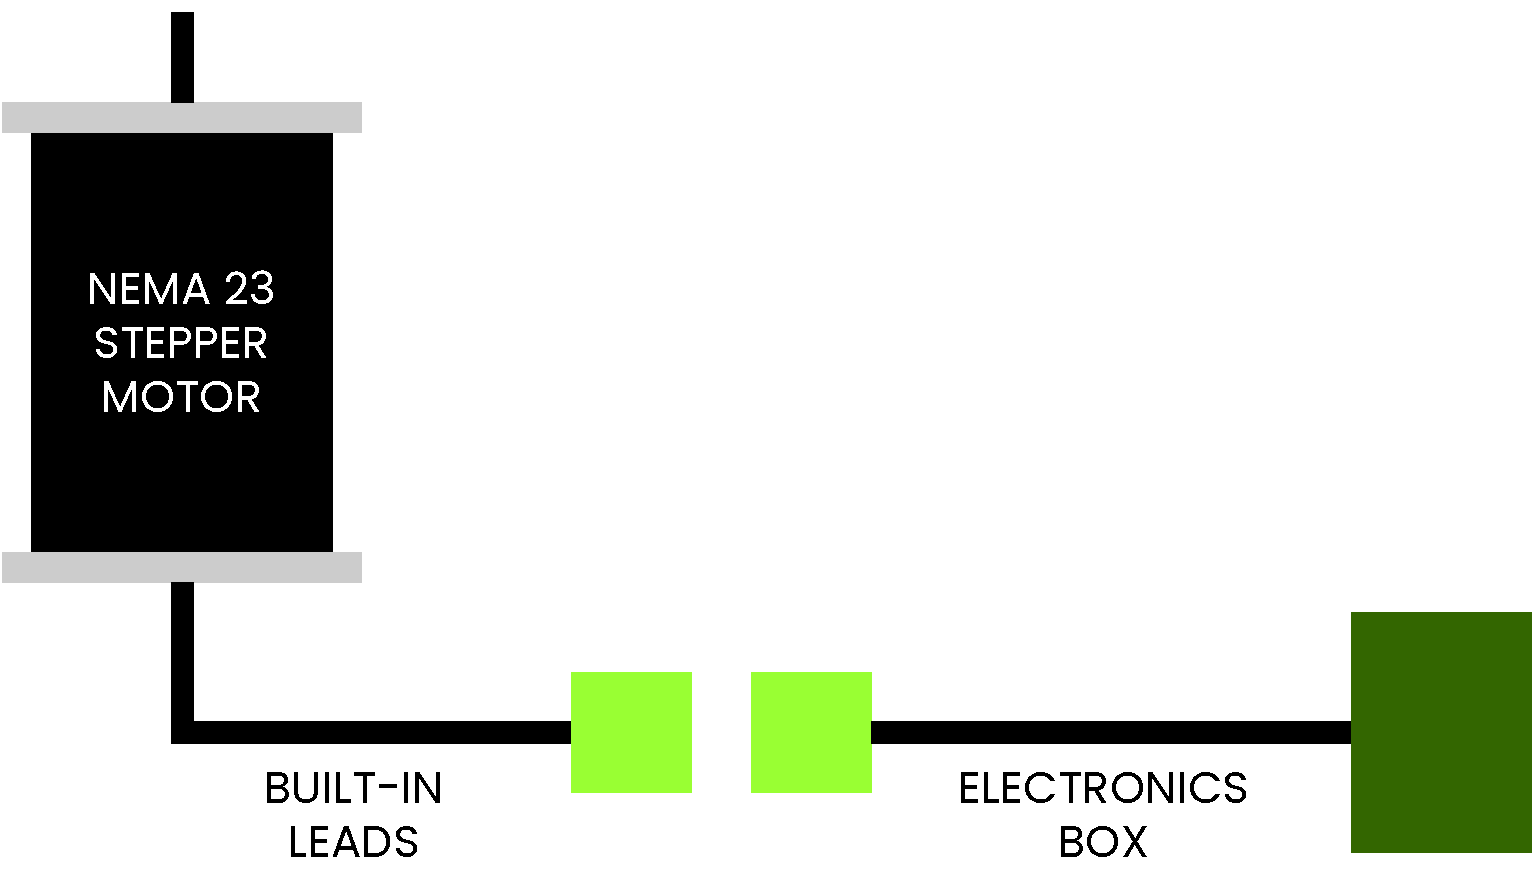
\includegraphics[width=0.4\textwidth]{images/cabling/y_axis_motors_cabling.pdf}
    \caption{Cabling stages for the Y-Axis motors.}
    \label{fig:cabling_y_axis_motors}
\end{figure}
The cabling for the Y-Axis motors consists of providing them with power from the electronics board to the motor themselves. The cabling should be done in such a way that its parts are located in the different major components. Figure \ref{fig:cabling_y_axis_motors} presents the cabling stages for the Y-Axis motors. A total of two (2) 4-pin connectors and 1750 millimeters of 4-phases cable are needed in order to execute the Y-Axis motors cabling. Table \ref{tab:cabling_y_axis_motors} presents the procedure for cabling the Y-Axis motors.

\begin{singlespace}
\begin{xltabular}{\textwidth}{|c|X|}
    
    \hline \multicolumn{2}{|c|}{\textbf{Y-Axis motors cabling}} \\ \hline
    \endhead
    
    \hline \multicolumn{2}{|c|}{\textbf{Y-Axis motors cabling}} \\ \hline
    \endfirsthead
    
    \multicolumn{2}{|c|}{\textit{Continues on next page.}} \\ \hline
    \endfoot
    
    \caption{Y-Axis motors cabling process.} \label{tab:cabling_y_axis_motors}
    \endlastfoot
    
    $\square$ & Peel the motors built-in cable tips. Solder or join the cable tips to the female side of one connector. Isolate the connections to prevent short-circuiting the motor phases. Repeat the process for both motors. \\ \hline
    $\square$ & Measure the distance between the cable opening at the side of both the left and right Y-Axis drivers and the electronics board. Measure the distance through the PVC tube and the cable opening of the electronics box. Cut two pieces of cable with the proper lengths. \\ \hline
    $\square$ & Peel the  electronics box cable tips. Pass the cable from the opening of the PVC tube until it reaches the electronics board inside the electronics box. Solder a male connector at the tip located in the PVC tube. Connect the other cable tip with the corresponding plug of the electronics board. \\ \hline
    $\square$ & Test the continuity of the cable from the electronics board plug to the male connector at the end of the cable. \\ \hline 
\end{xltabular}
\end{singlespace}

\subsection{Y-Axis Endstop Sensor}
\begin{figure}[H]
    \centering
    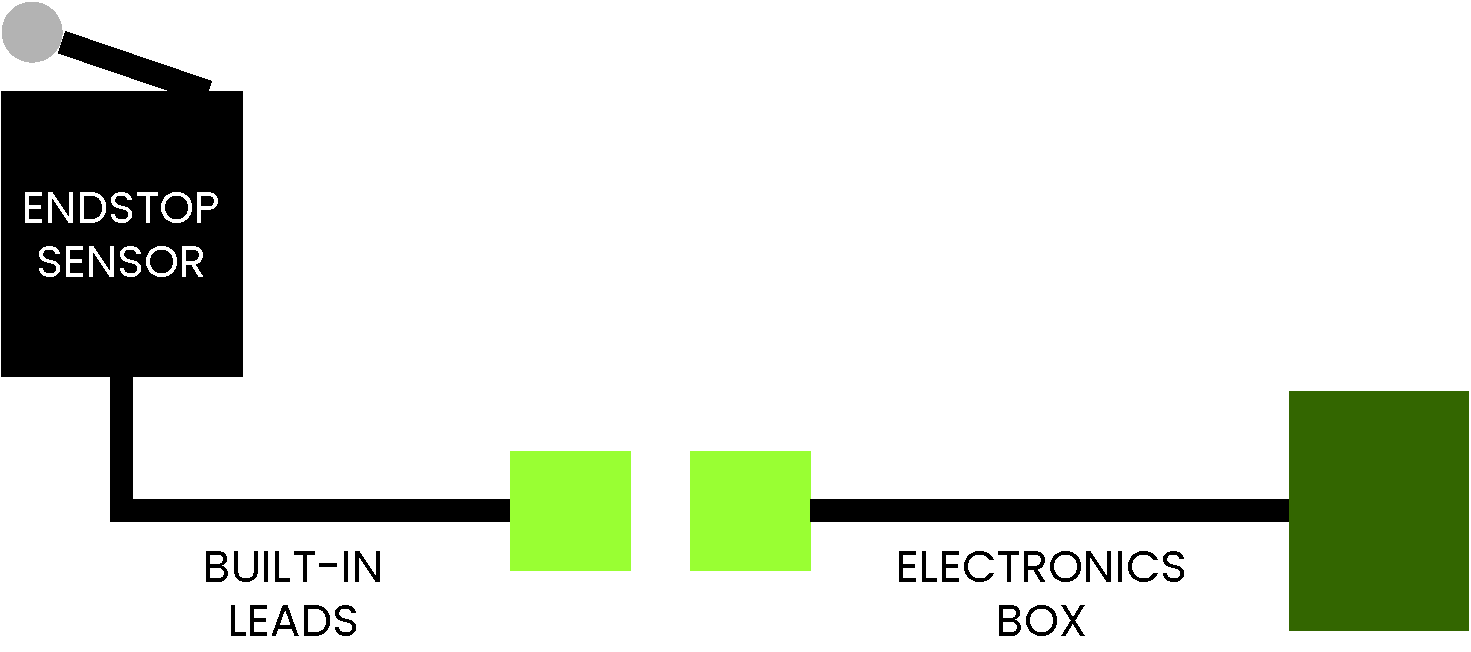
\includegraphics[width=0.4\textwidth]{images/cabling/y_axis_sensors_cabling.pdf}
    \caption{Cabling stages for the Y-Axis sensors.}
    \label{fig:cabling_y_axis_sensors}
\end{figure}
The cabling for the Y-Axis sensors consists of providing it with power from the electronics board to the sensor. The cabling should be done in such a way that its parts are located in the different major components. Figure \ref{fig:cabling_y_axis_sensors} presents the cabling stages for the Y-Axis sensor. A total of two (2) 3-pin connectors and 1050 millimeters of 3-phases cable are needed in order to execute the Y-Axis sensors cabling. Table \ref{tab:cabling_y_axis_sensors} presents the procedure for cabling the Y-Axis sensors.

\begin{singlespace}
\begin{xltabular}{\textwidth}{|c|X|}
    
    \hline \multicolumn{2}{|c|}{\textbf{Y-Axis endstop sensor cabling}} \\ \hline
    \endhead
    
    \hline \multicolumn{2}{|c|}{\textbf{Y-Axis endstop sensor cabling}} \\ \hline
    \endfirsthead
    
    \multicolumn{2}{|c|}{\textit{Continues on next page.}} \\ \hline
    \endfoot
    
    \caption{Y-Axis endstop sensor cabling process.} \label{tab:cabling_y_axis_sensors}
    \endlastfoot
    
    $\square$ & Peel the open end of the endstop sensor cable. Solder or join the cable tips to the female side of one connector. Isolate the connections to prevent short-circuiting the sensor cables. \\ \hline
    $\square$ & Measure the distance between the cable opening at the side of both the left Y-Axis driver and the electronics board. Measure the distance through the PVC tube and the cable opening of the electronics box. Cut two (2) pieces of cable with the proper lengths. \\ \hline
    $\square$ & Peel the  electronics box cable tips. Pass the cable from the opening of the PVC tube until it reaches the electronics board inside the electronics box. Solder a male connector at the tip located in the PVC tube. Connect the other cable tip with the corresponding plug of the electronics board. \\ \hline
    $\square$ & Test the continuity of the cable from the electronics board plug to the male connector at the end of the cable. \\ \hline 
\end{xltabular}
\end{singlespace}

\subsection{X-Axis Endstop Sensor}
\begin{figure}[H]
    \centering
    \includegraphics[width=0.6\textwidth]{images/cabling/x_axis_sensors_cabling.pdf}
    \caption{Cabling stages for the X-Axis endstop sensor.}
    \label{fig:cabling_x_axis_sensors}
\end{figure}
The cabling for the X-Axis sensors consists of providing it with power from the electronics board to the sensor. The cabling should be done in such a way that its parts are located in the different major components. Figure \ref{fig:cabling_x_axis_sensors} presents the cabling stages for the Y-Axis sensor. A total of three (2) 3-pin connectors and 2150 millimeters of 3-phases cable are needed in order to execute the X-Axis sensor cabling. Table \ref{tab:cabling_x_axis_sensors} presents the procedure for cabling the X-Axis sensors.

\begin{singlespace}
\begin{xltabular}{\textwidth}{|c|X|}
    
    \hline \multicolumn{2}{|c|}{\textbf{X-Axis endstop sensor cabling}} \\ \hline
    \endhead
    
    \hline \multicolumn{2}{|c|}{\textbf{X-Axis endstop sensor cabling}} \\ \hline
    \endfirsthead
    
    \multicolumn{2}{|c|}{\textit{Continues on next page.}} \\ \hline
    \endfoot
    
    \caption{X-Axis endstop sensor cabling process.} \label{tab:cabling_x_axis_sensors}
    \endlastfoot
    
    $\square$ & Peel the open end of the endstop sensor cable. Solder or join the cable tips to the female side of one connector. Isolate the connections to prevent short-circuiting the sensor cables. \\ \hline
    $\square$ & Measure the distance between the cable opening at the side of both the left Y-Axis driver and the electronics board. Measure the distance through the PVC tube and the cable opening of the electronics box. Cut a piece of cable with the proper length. This cable will run from the electronics board to the left Y-Axis driver. \\ \hline
    $\square$ & Peel the  electronics box cable tips. Pass the cable from the opening of the PVC tube until it reaches the electronics board inside the electronics box. Solder a male connector at the tip located in the PVC tube. Connect the other cable tip with the corresponding plug of the electronics board. \\ \hline
    $\square$ & Measure the distance between the cable opening for the electronics box PVC tube and the end link at the left Y-Axis driver. Cut a piece of cable with the proper length. \\ \hline
    $\square$ & Peel the cable tips and solder the connectors. The male connector will be located in the tip at the drag chain end, while the female at the cable opening for the PVC tube. \\ \hline
    $\square$ & Measure the distance along the Y-Axis drag chain. Cut a piece of cable of the proper length. \\ \hline
    $\square$ & Peel the tips of the cable and solder the connectors. A male connector will be located at the X-Axis driver end, while a female connector will be located in the drag chain end at the left Y-Axis driver. \\ \hline
    $\square$ & Peel the tips of a JST connector cable compatible with the endstop sensor. Solder a female connector at the tips of the cable. \\ \hline
    $\square$ & Plug the cable pieces together via the connectors. Make sure that all connections can remain together under some tension. \\ \hline
    $\square$ & Test the continuity of the cable from the electronics board plug to the male connector at the end of the cable. \\ \hline 
\end{xltabular}
\end{singlespace}

\subsection{Height Sensor}
\begin{figure}[H]
    \centering
    \includegraphics[width=0.9\textwidth]{images/cabling/height_sensors_cabling.pdf}
    \caption{Cabling stages for the height sensor.}
    \label{fig:cabling_height_sensors}
\end{figure}
The cabling for the height sensor consists of providing it with power from the electronics board to the sensor. The cabling should be done in such a way that its parts are located in the different major components. Figure \ref{fig:cabling_height_sensors} presents the cabling stages for the height sensor. A total of four (4) 3-pin connectors and 4350 millimeters of 3-phases cable are needed in order to execute the height sensor cabling. Table \ref{tab:cabling_height_sensor} presents the procedure for cabling the height sensor.

\begin{singlespace}
\begin{xltabular}{\textwidth}{|c|X|}
    
    \hline \multicolumn{2}{|c|}{\textbf{Height sensor cabling}} \\ \hline
    \endhead
    
    \hline \multicolumn{2}{|c|}{\textbf{Height sensor cabling}} \\ \hline
    \endfirsthead
    
    \multicolumn{2}{|c|}{\textit{Continues on next page.}} \\ \hline
    \endfoot
    
    \caption{Height sensor cabling process.} \label{tab:cabling_height_sensor}
    \endlastfoot
    
    $\square$ & Peel the height sensor JST cable. Solder or join the cable tips to the female side of one connector. Isolate the connections to prevent short-circuiting the motor phases. \\ \hline
    $\square$ & Measure the distance between the sensor connector and the X-Axis driver support through the X-Axis drag chain. This will be distance of the sensor cable from the GPR to the X-Axis driver. Make sure that cables are not under tension. Cut a piece of cable with the proper length. \\ \hline
    $\square$ & Pass the cable through the X-Axis drag chain. Peel the X-Axis cable tips and solder them to a male and female connector. The male connector will be used in the GPR side of the X-Axis drag chain. Keep in mind that the drag chain sides are not interchangeable. \\ \hline
    $\square$ & Measure the distance from the cable tip at the X-Axis driver support and the left Y-Axis driver trough the drag chain. This will be the cable distance from the X-Axis driver and the left Y-Axis driver. Remember to measure the distance through the drag chain. Cut a piece of cable with the proper length. \\ \hline
    $\square$ & Pass the cable through the Y-Axis drag chain. Peel the Y-Axis cable tips and solder them to a male and female connector. The male connector will be used in the X-Axis driver side of the Y-Axis drag chain. Keep in mind that the drag chains are not interchangeable. \\ \hline
    $\square$ & Measure the distance from the cable tip at the left Y-Axis driver support and the cable opening at support right side. You can use an auxiliary cable to measure that distance. Make sure to use the cable opening from the upper side of the support. Cut a piece of cable with the proper length. \\ \hline
    $\square$ & Pass the cable through the opening at the top of the left Y-Axis support. Peel the cable tips and solder a male and female connector at the tips. The male connector should be used to connect the cables at the end of the Y-Axis drag chain. \\ \hline
    $\square$ & Measure the distance between the cable opening at the side of the left Y-Axis driver and the electronics board. Measure the distance through the PVC tube and the cable opening of the electronics box. Cut a piece of cable with the proper length. \\ \hline
    $\square$ & Peel the  electronics box cable tips. Pass the cable from the opening of the PVC tube until it reaches the electronics board inside the electronics box. Solder a male connector at the tip located in the PVC tube. Connect the other cable tip with the corresponding plug of the electronics board. \\ \hline
    $\square$ & Test the continuity of the cable from the electronics board plug to the male connector from the X-Axis drag chain. Make sure that all the connectors are plugged. \\ \hline 
\end{xltabular}
\end{singlespace}

\subsection{VNA Power}
\begin{figure}[H]
    \centering
    \includegraphics[width=0.9\textwidth]{images/cabling/vna_power_cabling.pdf}
    \caption{Cabling stages for the VNA power.}
    \label{fig:cabling_vna_power}
\end{figure}
The cabling for the VNA power consists of providing the instrument with power from the power source to the VNA. The cabling should be done in such a way that its parts are located in the different major components. Figure \ref{fig:cabling_vna_power} presents the cabling stages for the VNA power. A total of four (4) AC plug connectors and 4350 millimeters of 3-phase AC cable are needed in order to execute the VNA power cabling. Table \ref{tab:cabling_vna_power} presents the procedure for cabling the VNA power.

\begin{singlespace}
\begin{xltabular}{\textwidth}{|c|X|}
    
    \hline \multicolumn{2}{|c|}{\textbf{VNA power cabling}} \\ \hline
    \endhead
    
    \hline \multicolumn{2}{|c|}{\textbf{VNA power cabling}} \\ \hline
    \endfirsthead
    
    \multicolumn{2}{|c|}{\textit{Continues on next page.}} \\ \hline
    \endfoot
    
    \caption{VNA power cabling process.} \label{tab:cabling_vna_power}
    \endlastfoot
    
    $\square$ & Measure the distance between the VNA AC plug connector and the X-Axis driver support through the X-Axis drag chain. This will be distance of the VNA power cable from the GPR to the X-Axis driver. Make sure that cables are not under tension. Cut a piece of cable with the proper length. \\ \hline
    $\square$ & Pass the cable through the X-Axis drag chain. Peel the X-Axis cable tips and solder them to a male and female connector. The male connector will be used in the GPR side of the X-Axis drag chain. Keep in mind that the drag chain sides are not interchangeable. \\ \hline
    $\square$ & Measure the distance from the cable tip at the X-Axis driver support and the left Y-Axis driver trough the drag chain. This will be the cable distance from the X-Axis driver and the left Y-Axis driver. Remember to measure the distance through the drag chain. Cut a piece of cable with the proper length. \\ \hline
    $\square$ & Pass the cable through the Y-Axis drag chain. Peel the Y-Axis cable tips and solder them to a male and female connector. The male connector will be used in the X-Axis driver side of the Y-Axis drag chain. Keep in mind that the drag chains are not interchangeable. \\ \hline
    $\square$ & Measure the distance from the cable tip at the left Y-Axis driver support and the cable opening at support right side. You can use an auxiliary cable to measure that distance. Make sure to use the cable opening from the upper side of the support. Cut a piece of cable with the proper length. \\ \hline
    $\square$ & Pass the cable through the opening at the top of the left Y-Axis support. Peel the cable tips and solder a male and female connector at the tips. The male connector should be used to connect the cables at the end of the Y-Axis drag chain. \\ \hline
    $\square$ & Measure the distance between the cable opening at the side of the left Y-Axis driver and the electronics board. Measure the distance through the PVC tube and the cable opening of the electronics box. Cut a piece of cable with the proper length. \\ \hline
    $\square$ & Peel the  electronics box cable tips. Pass the cable from the opening of the PVC tube until it reaches the electronics board inside the electronics box. Solder a male connector at the tip located in the PVC tube. The other tip will be used to connect the VNA power to the electricity source. \\ \hline
    $\square$ & Test the continuity of the cable from the electronics board plug to the plug at the GPR. Make sure that all the connectors are plugged. \\ \hline 
\end{xltabular}
\end{singlespace}

\subsection{VNA Data}
\begin{figure}[H]
    \centering
    \includegraphics[width=0.9\textwidth]{images/cabling/vna_data_cabling.pdf}
    \caption{Cabling stages for the VNA data.}
    \label{fig:cabling_vna_data}
\end{figure}
The cabling for the VNA data consists of providing it with an Ethernet connection from the network switch to the instrument. The cabling should be done in such a way that its parts are located in the different major components. Figure \ref{fig:cabling_vna_data} presents the cabling stages for the VNA data. A total of four (4) RJ-45 connectors and 4350 millimeters of Ethernet cable are needed in order to execute the VNA data cabling. Table \ref{tab:cabling_vna_data} presents the procedure for cabling the VNA data.

\begin{singlespace}
\begin{xltabular}{\textwidth}{|c|X|}
    
    \hline \multicolumn{2}{|c|}{\textbf{VNA data cabling}} \\ \hline
    \endhead
    
    \hline \multicolumn{2}{|c|}{\textbf{VNA data cabling}} \\ \hline
    \endfirsthead
    
    \multicolumn{2}{|c|}{\textit{Continues on next page.}} \\ \hline
    \endfoot
    
    \caption{VNA data cabling process.} \label{tab:cabling_vna_data}
    \endlastfoot
    
    $\square$ & Measure the distance between the motor connectors and the X-Axis driver support through the X-Axis drag chain. This will be distance of the motor cables from the GPR to the X-Axis driver. Make sure that cables are not under tension. Cut a piece of cable with the proper length. \\ \hline
    $\square$ & Pass the cable through the X-Axis drag chain. Punch RJ-45 plugs at the end of the cables. Then, check that the connectors can be used with the RJ-45 connectors. \\ \hline
    $\square$ & Measure the distance from the cable tip at the X-Axis driver support and the left Y-Axis driver trough the drag chain. This will be the cable distance from the X-Axis driver and the left Y-Axis driver. Remember to measure the distance through the drag chain. Cut a piece of cable with the proper length. \\ \hline
    $\square$ & Pass the cable through the Y-Axis drag chain. Punch RJ-45 plugs at the end of the cables. Then, check that the connectors can be used with the RJ-45 connectors.\\ \hline
    $\square$ & Measure the distance from the cable tip at the left Y-Axis driver support and the cable opening at support right side. You can use an auxiliary cable to measure that distance. Make sure to use the cable opening from the upper side of the support. Cut a piece of cable with the proper length. \\ \hline
    $\square$ & Pass the cable through the opening at the top of the left Y-Axis support. Punch RJ-45 plugs at the end of the cables. Then, check that the connectors can be used with the RJ-45 connectors. \\ \hline
    $\square$ & Measure the distance between the cable opening at the side of the left Y-Axis driver and the electronics board. Measure the distance through the PVC tube and the cable opening of the electronics box. Cut a piece of cable with the proper length. \\ \hline
    $\square$ & Peel the  electronics box cable tips. Punch RJ-45 plugs at the end of the cables. Then, check that the connectors can be used with the RJ-45 connectors. The tip at the electronics box will be used to connect the VNA data cable to the network switch. \\ \hline
    $\square$ & Test the network capabilities of the cable from the GPR to the electronics board. A network communication must be achieved in order for the communication to work. \\ \hline  
\end{xltabular}
\end{singlespace}

\newpage
\section{Robot First Time Configuration}
This section assumes that the robot basic assembly has been performed with the major components are assembled. Table \ref{tab:initial_status} presents the assumed status for each major component of the GPR-20 robot.

\begin{onehalfspacing}
    \begin{xltabular}{\textwidth}{|l|X|}
        \hline \textbf{Major Component} & \multicolumn{1}{c|}{\textbf{Status}} \\ \hline
        \endfirsthead
        
        \endhead
        
        \multicolumn{2}{|c|}{\textit{Continues on next page.}}
        \endfoot
        
        \caption{Initial status of the GPR-20 major components.} \label{tab:initial_status}
        \endlastfoot
        
        Electronics Box & The whole electronics box is assembled. Voltage converters, on-board computer and electronics PCB are assumed to be installed although without the major connections performed. Electronic components are not installed in the electronic box. \\ \hline
        Y-Axes & Both axes are assembled. The two motors and an endstop sensor are installed in each driver component. Motor and sensor cables do not have a plug connected at its end. Two (2) drag chain ends are attached to left Y-Axis extender and the X-Axis driver. \\ \hline
        X-Axis & The axis is fully assembled. No motors or electronic components are required for this assembly. \\ \hline
        VNA Holder & The VNA holder is fully assembled. Neither the antennae nor the Vector Network Analyzer are installed in the assembly. The IR height measurement sensor is installed. No cable extender nor plugs are connected to the IR height sensor. \\ \hline
        Ground Support & Four ground support elements are fully assembled. \\ \hline
    \end{xltabular}
\end{onehalfspacing}

\subsection{Electronics Box First Time Configuration}
The electronics box first time configuration consists of installing the electronic components into the board. Figure \ref{fig:electronics_board} presents the electronics board layout. Components and connectors of the board are indicated in the diagram. Do not install the electronic components directly into the board. Use sockets to provide the connection between the components and the board. The board with the installed sockets is presented in figure \ref{fig:electronics_socket}.

\begin{figure}[H]
    \centering
    \includegraphics[width=0.8\textwidth]{images/first_time/board.png}
    \caption{Electronics board with the components.}
    \label{fig:electronics_board}
\end{figure}

\begin{figure}[H]
    \centering
    \includegraphics[width=0.8\textwidth]{images/first_time/PCB_mkII.jpg}
    \caption{Manufactured electronics board with the socket installed.}
    \label{fig:electronics_socket}
\end{figure}

\subsection{Personal Computer First Time Configuration}
The personal computer setup consists of installing and configuring the required software for it to be run on it. The procedure is presented in table \ref{tab:personal_computer}.

\begin{onehalfspacing}
    \begin{xltabular}{\linewidth}{|c|X|}
        
        \hline & \textbf{Description} \\ \hline
        \endfirsthead
        
        \hline & \textbf{Description} \\ \hline
        \endhead
        
        \multicolumn{2}{|c|}{\textit{Continues on next page.}} \\ \hline
        \endfoot
        
        \caption{Steps for installing the software tools in the personal computer.} \label{tab:personal_computer}
        \endlastfoot
    
        1 & Install the latest version of Ubuntu. The version used for the robot development is 20.04LTS. Instructions on the OS installation depend on the computer model. \\ \hline
        2 & Install Robotic Operating System (ROS). The ROS version depends on the OS version that was installed in the previous step. The version used for the robot development is ROS Noetic. \\ \hline
        3 & Create a folder in the \texttt{home} directory of the personal computer. The name of the folder should be \texttt{gpr20\_ws}. Create an additional folder inside with the \texttt{src} name. \\ \hline
        4 & Initialize the workspace by executing the \texttt{\$ catkin\_make} command. Make sure that the current directory is \texttt{gpr20\_ws} folder. \\ \hline
        5 & Download the \texttt{gpr20\_msgs}, \texttt{gpr20\_vna\_acquisition} and \texttt{gpr20\_vna\_processing} repositories inside the \texttt{src} folder of the \texttt{gpr20\_ws} directory. \\ \hline
        6 & Execute the \texttt{catkin\_make} command again in the \texttt{gpr20\_src} directory. \\ \hline
    \end{xltabular}
\end{onehalfspacing}

\subsection{Network Switch First Time Configuration}
The network switch configuration consists of setting up the device in order to prevent it from broadcasting a wireless network. The procedure generally consists of the steps presented in table \ref{tab:network}. However, specific details should be consulted in the user manual of the network switch.

\begin{onehalfspacing}
    \begin{xltabular}{\linewidth}{|c|X|}
        
        \hline & \textbf{Description} \\ \hline
        \endfirsthead
        
        \hline & \textbf{Description} \\ \hline
        \endhead
        
        \multicolumn{2}{|c|}{\textit{Continues on next page.}} \\ \hline
        \endfoot
        
        \caption{Steps for removing the broadcasting of the wireless network of the switch.} \label{tab:network}
        \endlastfoot
    
        1 & Turn on the network switch and connect it to a computer via a Ethernet cable. \\ \hline
        2 & Access the network switch configuration panel via a web browser. The address of the network switch generally is \texttt{192.168.0.1}, however it can be consulted using third party tools designed to identify devices over a network. \\ \hline
        3 & Login into the configuration panel. The credentials are usually located in either the back or bottom of the network switch. \\ \hline
        4 & Access the wireless configuration of the network switch. Disable the broadcast of the wireless network or networks. Save the configuration. \\ \hline
        5 & Log out of the configuration panel. \\ \hline
    \end{xltabular}
\end{onehalfspacing}


\end{document}
